\documentclass[aoas,preprint]{imsart}
%\RequirePackage{mdframed}
%\usepackage{mdframed}
\usepackage[framemethod=TikZ]{mdframed}
\RequirePackage[OT1]{fontenc}
\usepackage[utf8x]{inputenc}
\RequirePackage{amsthm,amsmath}
\RequirePackage{natbib}
\RequirePackage[colorlinks,citecolor=blue,urlcolor=blue]{hyperref}

\usepackage[sc]{mathpazo}
\usepackage{amsmath, wrapfig}
\usepackage{dsfont}
\usepackage{graphicx}
\usepackage{caption}
\usepackage{flafter}
\usepackage[section]{placeins}
\DeclareCaptionFormat{myformat}{\hrulefill \\ #1#2#3}
\DeclareCaptionFont{small}{\footnotesize}
\DeclareCaptionFont{blue}{\color{blue}} 
\DeclareCaptionFont{bf}{\bfseries}
\renewcommand{\tablename}{Appendix Table}
\renewcommand{\thetable}{A\arabic{table}}
\captionsetup[figure]{format=myformat,labelfont={blue,bf,small},font=small}
\usepackage{booktabs}% http://ctan.org/pkg/booktabs

%\usepackage{algorithm,algcompatible,amsmath}
\usepackage{algorithm, eqparbox,array}% http://ctan.org/pkg/algorithms
\usepackage{algpseudocode}% http://ctan.org/pkg/algorithmicx
%\usepackage{xcolor}
%\usepackage[usenames, dvipsnames]{color}
\usepackage{color}
\RequirePackage{xcolor}
%\usepackage{mdframed}

%%%% next line added by Keegan for easy commenting; feel free to remove!
\usepackage[colorinlistoftodos]{todonotes}


%\documentclass[11pt]{amsart}
%\usepackage{geometry,amsmath,amssymb,amsthm,cite,mathtools,float, caption, comment}                % See geometry.pdf to learn the layout options. There are lots.
%%\usepackage[numbers, sort&compress]{natbib}
%\usepackage[authoryear,sort]{natbib}
%\bibliographystyle{plainnat}
%\geometry{letterpaper}                   % ... or a4paper or a5paper or ... 
%%\geometry{landscape}                % Activate for for rotated page geometry
%%\usepackage[parfill]{parskip}    % Activate to begin paragraphs with an empty line rather than an indent
%\usepackage{graphicx}
%\usepackage{algorithm}
%\usepackage[noend]{algpseudocode}
%\usepackage{amssymb}
%\usepackage{epstopdf}
%\usepackage[parfill]{parskip}

 \setlength{\parskip}{1ex}
\newtheorem{lemma}{Lemma}
\newtheorem{theorem}{Theorem}
\newtheorem{prop}{Proposition}
\DeclareGraphicsRule{.tif}{png}{.png}{`convert #1 `dirname #1`/`basename #1 .tif`.png}

\begin{document}

\begin{frontmatter}
\title{A compositional model to assess expression changes from
 single-cell RNA-seq data}

\begin{aug}

\author{\fnms{Xiuyu} \snm{Ma}\thanksref{t1}\ead[label=e1]{ma79@wisc.edu}},
\author{\fnms{Keegan} \snm{Korthauer}\thanksref{k1,k2}\ead[label=e2]{keegan@jimmy.harvard.edu}},
\author{\fnms{Christina} \snm{Kendziorski}\thanksref{t2}\ead[label=e2]{kendzior@biostat.wisc.edu}},
\and
\author{\fnms{Michael} \snm{Newton}\thanksref{t1,t2}
\ead[label=e3]{newton@stat.wisc.edu}
\ead[label=u1,url]{http://www.foo.com}}

\affiliation{Department of Statistics\thanksmark{t1}, 
Department of Biostatistics and Medical Informatics\thanksmark{t2}, University of Wisconsin - Madison;
Department of Data Sciences, Dana-Farber Cancer Institute\thanksmark{k1};
Department of Biostatistics, Harvard T.H. Chan School of Public Health\thanksmark{k2}}

\address{Address of the First and Second authors\\
Usually a few lines long\\
\printead{e1}\\
\phantom{E-mail:\ }\printead*{e2}}

\address{Address of the Third author\\
Usually a few lines long\\
Usually a few lines long\\
\printead{e3}\\
\printead{u1}}


\end{aug}


\begin{abstract}
On the problem of scoring genes for evidence of changes in the distribution of single-cell expression, we
introduce a empirical Bayesian mixture approach and evaluate its operating characteristics 
in a range of numerical experiments.  The proposed approach leverages cell-subtype 
structure revealed in cluster analysis in order to boost gene-level information on expression changes.
Cell clustering informs gene-level analysis through a specially-constructed prior distribution
over pairs of multinomial probability vectors; this prior meshes with available model-based tools
that score patterns of differential expression over multiple subtypes.   
We derive an explicit formula for the posterior probability that a gene has the same distribution
in two cellular conditions, allowing for a gene-specific mixture over subtypes in each condition.
Advantage is gained by the compositional structure of the model, in which a host of gene-specific
mixture components are allowed, but also in which the mixing proportions are constrained at the whole 
cell level.  This structure leads to a novel form of information sharing through which the cell-clustering
results support gene-level scoring of differential distribution.  The result, according to our
numerical experiments, is improved sensitivity compared to several standard approaches
 for detecting distributional expression changes.  
\end{abstract}

%\maketitle
\end{frontmatter}

\section{Introduction}

The ability to measure genome-wide gene expression at single-cell resolution 
has accelerated the pace of biological discovery.  Overcoming data
analysis challenges caused by the scale and unique variation properties of single-cell
data will surely fuel further advances in immunology \citep{immune}, developmental
biology \citep{dv}, cancer \citep{cancer}, and other areas \citep{scs}. 
 Computational tools and statistical methodologies 
created for data of lower-resolution (e.g., bulk RNA-seq) or lower dimension 
(e.g., flow cytometry)  guide our response to 
 the data science demands of new measurement platforms,
but they remain inadequate for efficient knowledge discovery in this
rapidly advancing domain~\citep{Bacher2016}.

An important feature of single-cell studies that could be leveraged better
statistically is the fact that cells populate distinct, identifiable subtypes
determined by lineage history, epigenetic state, the activity
of various transcriptional programs, or other 
distinguishing factors. Extensive research on clustering cells
has produced tools for identifying subtypes, including: 
 \verb+SC3+ \citep{sc3}, \verb+CIDR+ \citep{CIDR} and \verb+ZIFA+ \citep{ZIFA}.
We hypothesize that such
subtype information may be usefully injected into other inference procedures in order
to improve their operating characteristics. 

Assessing the magnitude and statistical significance of changes in gene
expression associated with changes in cellular condition has been a central
statistical problem in genomics. New tools specific to
the single-cell RNAseq data structure, including \verb+MAST+
\citep{ref:MAST}, \verb+scDD+ \citep{ref:scDD}, \verb+D3E+ \citep{ref:d3e},
have been deployed to address this problem.
These tools respond
to scRNAseq characteristics, such as high prevelance of zero counts and
gene-level multimodality, but they do not fully exploit cellular-subtype
information.  We address this limitation, aiming to increase power to detect differential distribution.
The proposed method measures changes in a gene's marginal mixture distribution, and
acquires sensitivity to a wide variety of distributional effects by how it integrates commonalities gene-level data for learned cellular subtypes.  It is implemented in  software 
in the R package \verb+scDDboost+~\footnote{http://github.com/wiscstatman/scDDboost/}.
Modularity in the necessary elements provides some methodological advantages. For example,
improvements in clustering may be used in place of the default clustering
without altering the form of downstream analysis.  Also, by avoiding Markov chain Monte Carlo,
\verb+scDDboost+ computations are relatively inexpensive for a Bayesian procedure.

Through the compositional model underlying \verb+scDDboost+, subtypes inferred by clustering 
inform the analysis of gene-level expression.  The proposed methodology merges two lines of computation
after cell clustering: one concerns patterns of differential expression among 
the cellular subtypes, and here we take advantage of the powerful \verb+EBseq+ method for detecting
patterns in negative-binomially-distributed expression data~\citep{ref:oscope}.  The second concerns 
the counts of cells in various subtypes; for this we propose a Double-Dirichlet-Mixture distribution
to model the pair of multinomial probability vectors for subtype counts in two experimental conditions.
Further elements are developed, on the selection of the number of subtypes and on accounting for uncertainty in the cluster output,  in order to provide an end-to-end solution to the differential distribution
problem.

To set the context by way of example, 
Figure~\ref{fig:whet} highlights the ability of \verb+scDDboost+ to detect subtype composition changes that lead to subtle gene expression changes that go undetected by other methods. 
The three panels on the left compare expression from 91 human 
stem cells known to be in the G1 phase of the cell cycle, as well as
from 76 such cells known to be in the G2/M phase~\citep{ref:Leng} in three genes (BIRC5, HMMR, and CKAP2), which we happen to know from prior studies have differential activity between G1 and G2/M~\citep{BIRC5,HMMR,RAD21}.  
Standard statistical tools \todo{which standard statistical tools?} applied to the data behind Figure~\ref{fig:whet} do not find the observed
 differences in any of these genes
to be statistically significant when controlling the false discovery rate (FDR) at 5\%. 
But \verb+scDDboost+ does include these genes on its 5\% FDR list.
Considering prior studies, these subtle distributional changes are probably not false discoveries. \todo{From the heatmap, these genes look
to be srikingly bimodal. But I don't get that sense from the violin plots. Are the same transformations, treatment of dropouts used for both panels? Perhaps it would help to see the color scale legend for the heatmap?}
The right panel in Figure~\ref{fig:whet} shows these three among
  many other genes also known to be involved in cell-cycle regulation but
not identified by standard tools as altered between G1 and G2/M at the 5\% FDR level.    The color panel above the
heatmap hints at why \verb+scDDboost+ has identified these genes. Cells (columns) are clustered by their genome-wide
expression profiles into distinct cellular subtypes, as indicated by the color panel.   Evidently, these 
subtypes have changed in their proportions between G1 and G2/M; for instance, there is a lower proportion
 of {\em red} cells and a greater proportion of {\em orange} cells in G2/M. These proportion shifts, 
inferred from genome-wide data, infuse information into gene-specific tests which measure 
changes between conditions in the mixture distribution of expression.  We note that \verb+scDDboost+ 
agrees with other statistical tools on very strong differential-distribution signals (not shown), but it 
has the potential to increase power for subtle signals owing to its unique approach to leveraging cell subtype
information.



\begin{figure}[H]
%\vspace{-\parskip}
%\minipage{0.36\textwidth}
%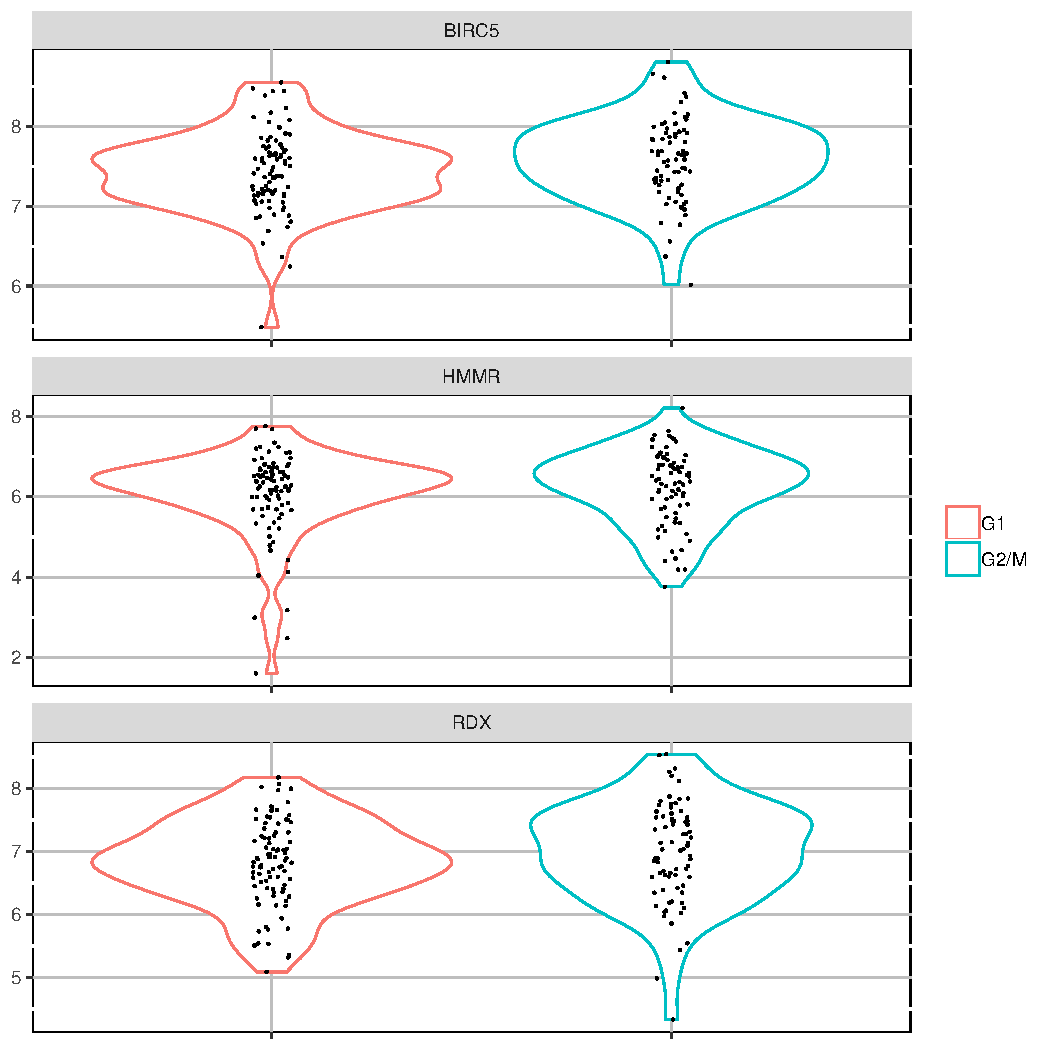
\includegraphics[clip,width=\textwidth]{Figs/FucciDD.pdf}
%\endminipage
%\minipage{0.64\textwidth}
 %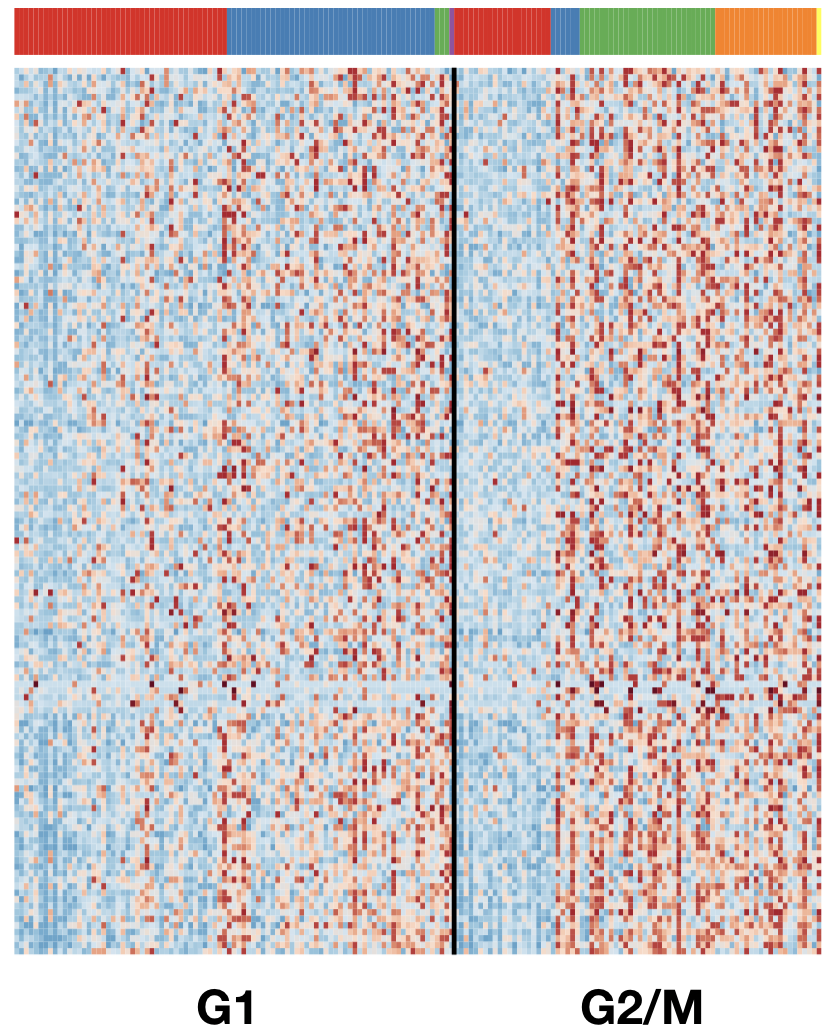
\includegraphics[clip,width=\textwidth]{Figs/HeatUni.png}
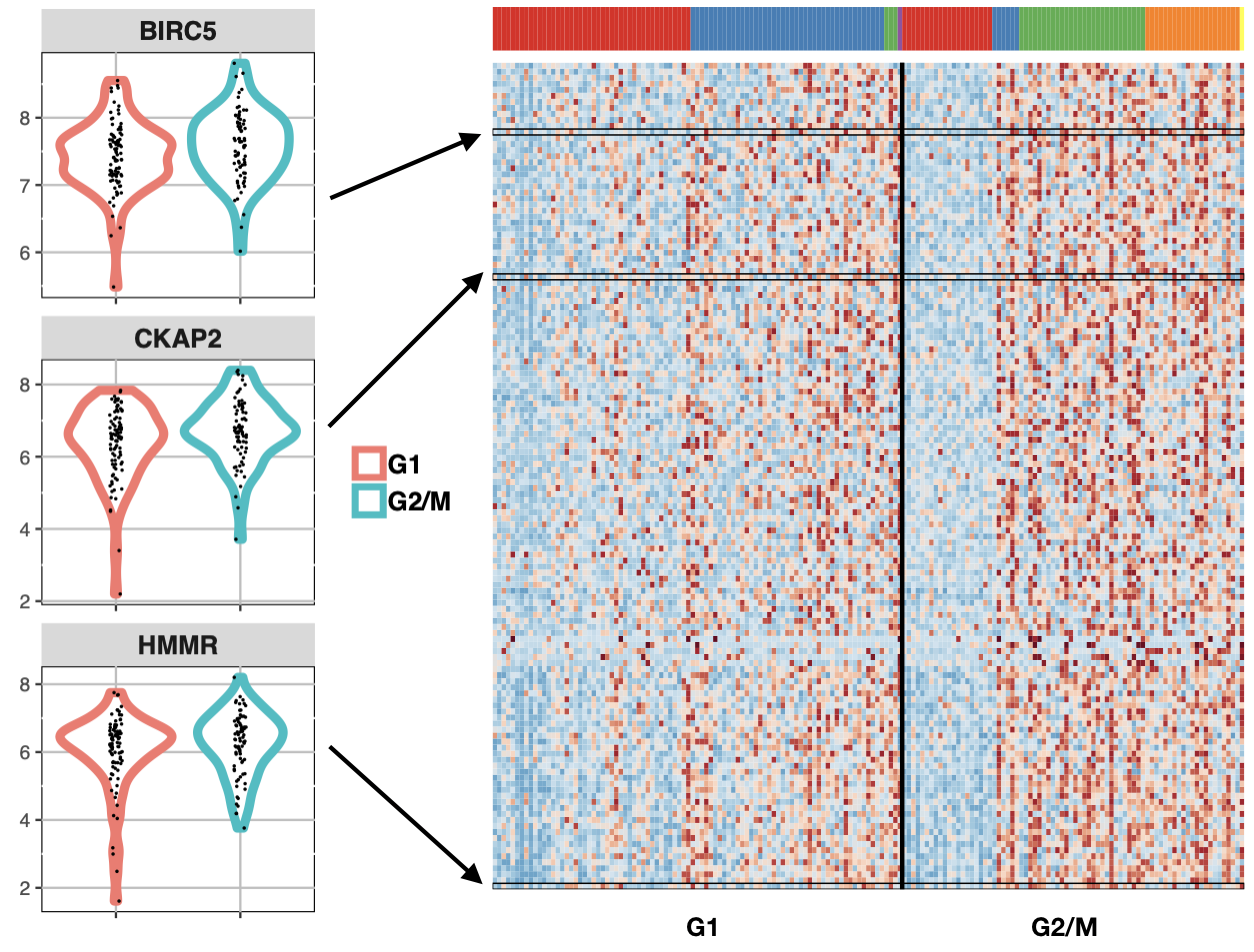
\includegraphics[width=\textwidth]{Figs/Fig1.png}
%\endminipage

 \caption{Genes involved in cell-cycle that are identified by scDDboost, but not standard approaches,
 as differentially distributed between cell-cycle phases G1 and G2/M in human embryonic stem cells. 
  Density estimates on the left show expression data (log2 scale)
of three genes identified by scDDboost at 5\% FDR, but not similarly identified by other approaches.
 Prior studies have shown that the expression
 of  BIRC5, CKAP2, and HMMR is dependent on the phase of cell-cycle,
 suggesting that these subtle shifts are not false positives. 
 Heatmap (right) shows these three genes among 137 other cell-cycle genes (GO:0007049). 
 Cells (columns) are clustered by their genome-wide
expression profiles into distinct cellular subtypes, as indicated by the color panel. 


 \label{fig:whet} }
\end{figure}


\todo{Fig 1(left): Where are the dropouts? Was a pseudocount used?}
\todo{Fig 1(right): Missing legend for color scale}
Numerical experiments  on both synthetic and published scRNA-seq data bear out the incidental finding 
in Figure~\ref{fig:whet}, that \verb+scDDboost+ has sensitivity for detecting subtle distribution changes. 
  In these experiments we take advantage of
\verb+splatter+ for generating synthetic data~\citep{ref:Zappia} as well as the compendium of scRNA-seq
data available through \verb+conquer+ \citep{ref:Cq}.  Additional numerical experiments show a relationship
 between \verb+scDDboost+ findings and more mechanistic attempts to parameterize transcriptional
 activation~\citep{ref:d3e}.  Finally, we establish first-order asymptotic results for the methodology.  

On manuscript organization, we present
the modeling and methodology elements in Section~2, numerical experiments in Section~3,  asymptotic analysis in Section~4, and a discussion
in Section~5.  We relegate some details to an appendix and many others to a Supplementary 
Material document.



\section{Modeling}
\subsection{Data structure, sampling model, and parameters}

In modeling scRNASeq data, we
imagine that each cell $c$ falls into one of $K>1$ classes, which we think of as
subtypes or subpopulations of cells. For notation, $z_c=k$ means that cell $c$ happens to be of subtype $k$, with the vector $z=(z_c)$ recording
the states of all sampled cells.  Knowledge of this class structure
 prior to measurement is not required, as it will be inferred as necessary from
 available genomic data.   We expect that cells arise from multiple
experimental conditions, such as by treatment-control status or some other factors
 measured at the cell level, but we present our development for the special
case of two conditions.  Notationally, $y=(y_c)$ records the experimental condition, say $y_c=1$ or $y_c=2$.
 Let's say condition $j$ measures $n_j=\sum_{c} 1[y_c=j]$ cells,  and
in total we have $n=n_1+n_2$ cells in the analysis.  The examples in Section~3 involve hundreds to thousands of cells.
Further let \begin{eqnarray}
\label{eq:counts}
t^j_k = t^j_k(y,z) = \sum_c 1[y_c=j, z_c=k] 
\end{eqnarray}
denote the number of cells of subtype $k$ in condition $j$;
we infer something about these counts using genome-wide data.  As for molecular data, the 
normalized expression of gene $g$ in cell $c$, say $X_{g,c}$, is one entry
in a typically large {\sc{genes}} by {\sc{cells}} data matrix $X$.  Thus, the data structure entails an expression matrix
$X$, a treatment label vector $y$, and a vector $z$ of latent subtype labels.


We treat subtype counts in the two conditions,  $t^1 = (t^1_1, t^1_2, \cdots, t^1_K )$ and 
$t^2 = (t^2_1, t^2_2, \cdots, t^2_K)$,  as independent multinomial
vectors, reflecting the experimental design.  Explicitly,
\begin{eqnarray}
\label{eq:mult}
t^1| y \sim \text{Multinomial}_K( n_1, \phi ) \quad {\mbox {\rm and}} \quad
t^2| y \sim \text{Multinomial}_K( n_2, \psi )
\end{eqnarray}
for probability vectors 
$\phi = (\phi_1, \phi_2, \cdots, \phi_K)$ and 
 $\psi = ( \psi_1, \psi_2, \cdots, \psi_K)$ that characterize the populations of
cells from which the $n$ observed cells are sampled.  This follows from the more basic 
sampling model:
$P(z_c=k|y_c=1) = \phi_k$ and $P(z_c=k| y_c =2 ) = \psi_k.$

Our working hypothesis, referred to as the {\em compositional model},  is that any differences in the distribution of expression $X_{g,c}$ 
between $y_c=1$ and $y_c=2$ (i.e., any condition effects) are attributable 
to differences between the conditions 
in the underlying composition of cell types; i.e.,
owing to $\phi \neq \psi$.  We suppose that cells of any given subtype $k$ will
present data according to a distribution reflecting technical 
and biological variation specific to that class of cells, regardless of the 
condition the cell finds itself in.   Some care is needed in this, as an overly
broad cell subtype (e.g., {\em epithelial cells}) could have
further subtypes that show differential response to some treatment, for example,
and so cellular condition (treatment) would then affect the distribution of 
expression data within the subtype, which is contrary to our working hypothesis.
Were that the case,  we could have refined the subtype definition to allow a greater
number of population classes $K$ in order to mitigate the problem of within-subtype 
heterogeneity. A  risk in this approach is that $K$ could approach $n$, as if  
every cell were  its own subtype.  We find, however,
that data sets often encountered do not display this theoretical phenomenon
when considering a broad class of within-subtype expression distributions.
We revisit the issue in Section~4, but for now we proceed assuming 
that cellular condition affects the composition of subtypes but not the distribution of expression
within a subtype.

Within the compositional model, let $f_{g,k}$ denote the sampling distribution
of expression measurement $X_{g,c}$ assuming that cell $c$ is from subtype $k$.
Then for the two cellular conditions, and at some expression level $x$, 
the marginal distributions over subtypes are finite mixtures:
\begin{eqnarray*}
f_g^1(x) = \sum_{k=1}^K \phi_k f_{g,k} (x) \quad {\mbox {\rm and}} \quad
f_g^2(x) = \sum_{k=1}^K \psi_k f_{g,k} (x).
\end{eqnarray*}
In other words,  $X_{g,c} |[ y_c=j]  \sim f_g^j$  and $X_{g,c} |[ z_c=k, y_c=j] \sim f_{g,k}$.

We say that gene $g$ is {\em differentially distributed}, denote ${\rm DD}_g$ and indicated
$f_g^1 \neq f_g^2$,
if $f_g^1(x) \neq f_g^2(x)$ for some $x$, and otherwise it is equivalently distributed
(${\rm ED}_g$). Motivated by findings from bulk RNAseq data analysis, we further
set each $f_{g,k}$ to have a a negative-binomial form, say with mean $\mu_{g,k}$
and shape parameter $\sigma_g$; e.g. \cite{ref:Leng}, \cite{DES}, and \cite{ref:Des}. 
This choice is effective in our numerical experiments though it is 
not critical to the modeling formulation.  The use of mixtures per gene has proven
useful in related model-based approaches (e.g., 
\cite{ref:MAST}; \cite{McDavid:2014aa}; \cite{Huang:2018aa}).
Our perspective is that  genome-wide data may usefully inform the  mixing proportions.

We seek methodology to prioritize genes for evidence
of ${\rm DD}_g$.  Interestingly, even if we have evidence for condition effects
on the subtype frequencies, it does not follow that a given
gene will have $f^1_g \neq f^2_g$; that depends on whether or not the subtypes
show the right pattern of {\em differential expression} at $g$, to use the 
standard terminology from bulk RNAseq.  For example, if two subtypes have 
different frequencies between the two conditions ($\phi_1 \neq \psi_1$ and 
 $\phi_2 \neq \psi_2$) but the same aggregate frequency
($\phi_1+\phi_2 = \psi_1 + \psi_2$),  and also  if $\mu_{g,1} = \mu_{g,2}$
then, other things being equal, $f^1_g = f^2_g$ even though $\phi \neq \psi$. The fact
is so central that we emphasize:


\noindent
{\bf Key issue:} A gene that does not distinguish two subtypes will also not distinguish
the cellular conditions if those subtypes appear in the same aggregate frequency
in the two conditions, regardless of changes in the individual subtype 
frequencies. 

 We formalize this issue in order that our methodology
has the necessary functionality.  To do so,  first consider the parameter space 
$\Theta = \{ \theta=(\phi, \psi,\mu, \sigma)  \}$,
where $\phi=(\phi_1, \phi_2, \cdots, \phi_K)$ and $\psi=(\psi_1, \psi_2, \cdots, \psi_K)$ 
are as before, where $\mu = \{ \mu_{g,k} \}$ holds  all the subtype-and-gene-specific expected
values, and where $\sigma = \{ \sigma_g \}$ holds all the gene-specific negative-binomial
shape parameters.  Critical to our construction are special subsets of $\Theta$ corresponding
to partitions of the $K$ cell subtypes.  A single partition, $\pi$, is a set of
mutually exclusive and exhaustive blocks, $b$, where each block is a subset of $\{1, 2, 
\cdots, K\}$, and we write $\pi = \{ b \}$.  Of course,
the set $\Pi$ containing all partitions $\pi$ of $\{1,2, \cdots, K\}$
 has cardinality that grows rapidly with $K$. 
 We carry along an example
involving $K=7$ cell types, and one three-block partition taken
from the set of 877 possible partitions of $\{1, 2, \cdots, 7\}$ (Figure~\ref{fig:scheme}).

\begin{figure}[h!]
  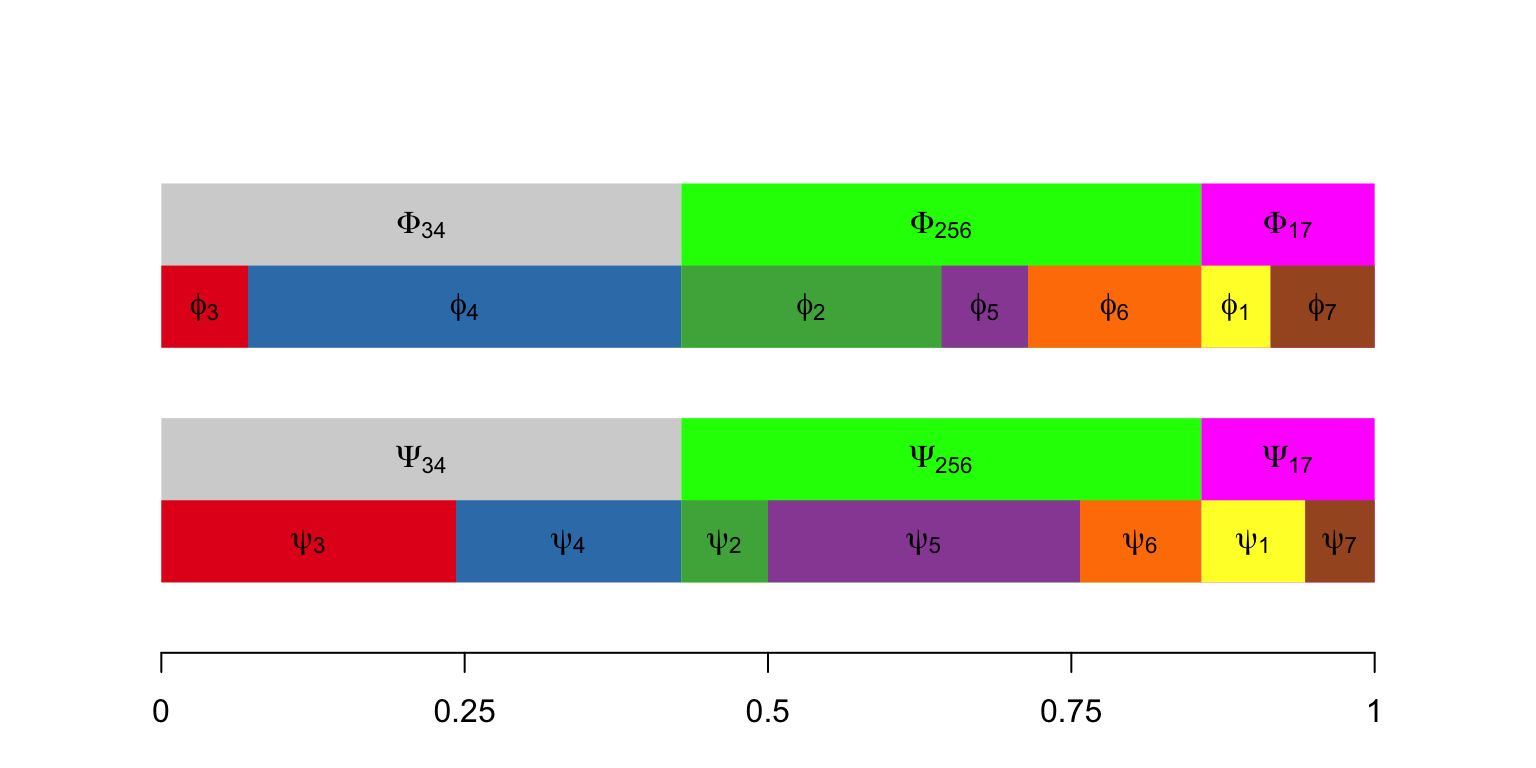
\includegraphics[width=\linewidth]{Figs/schematic-1.png}
  \caption{Proportions of $K=7$ cellular subtypes in different conditions. 
 Aggregated proportions of subtypes 3 and 4, subtypes 2, 5, and 6, and subtypes 1, and 7 
 remain same across conditions, while individual subtype frequencies change. 
 Depending on the changes in average expression among subtypes, these frequency changes
may or may not induce changes between two conditions  in the  marginal distribution of some gene's expression.  }
  \label{fig:scheme}
\end{figure}


For any partition $\pi=\{b\}$, consider aggregate subtype frequencies
\begin{eqnarray*}
\Phi_b = \sum_{k\in b} \phi_k \quad {\mbox {\rm  and}} \quad 
 \Psi_b = \sum_{k\in b} \psi_k,
\end{eqnarray*}
and extend the notation, allowing vectors $\Phi_\pi = \{ \Phi_b: b \in \pi \}$ and similarly
for $\Psi_\pi$. Recall the partial ordering of partitions based on refinement, and note that
as long as $\pi$ is not the most refined partition (every cell type its own block),
then the mapping from $( \phi, \psi )$ to $( \Phi_\pi, \Psi_\pi)$ is many-to-one.
Further, define sets
\begin{eqnarray}
\label{eq:asets}
A_\pi = \{ \theta\in \Theta: \; \Phi_b = \Psi_b  \, \forall b \in \pi \}.
\end{eqnarray}
and
\begin{eqnarray}
\label{eq:msets}
M_{g,\pi} = \{ \theta \in \Theta: \; \mu_{g,k} = \mu_{g,k'} \iff k,k' \in b, b \in \pi \}.
\end{eqnarray}
Under $A_\pi$ there are constraints on cell subtype frequencies; under $M_{g,\pi}$ there is 
equivalence in the gene-level distribution of expression between certain subtypes.
These sets are precisely the
structures needed to address differential distribution DD$_g$ (and
it complement, equivalent distribution, ${\rm ED}_g$) at a given gene
$g$, since:

\begin{theorem}  Let $C_{g,\pi} = A_\pi\cap M_{g, \pi}$.  For 
partitions $\pi_1 \neq\pi_2$, \mbox{$C_{g,\pi_1} \cap C_{g,\pi_2} = \emptyset$}. Further,
 at any gene $g$, equivalent distribution is
\begin{eqnarray*}
{\rm{ED}}_g = \bigcup_{\pi \in \Pi} C_{g,\pi}.
\end{eqnarray*}
\end{theorem}
With additional 
probability structure on the parameter space,  we immediately obtain from Theorem~1 
a formula for local false discovery rates:
\begin{align}
\label{eq:lfdr}
1-P(\text{DD}_g|X,y) = 
 P(\text{ED}_g|X,y) = \sum_{\pi \in \Pi} P\left(A_\pi \cap M_{g,\pi} |X,y \right).
\end{align}
Such local false discovery rates are important empirical Bayesian 
statistics in large-scale testing (\cite{Efron:2007aa}; \cite{Muralidharan:2010aa}; \cite{Newton:2004aa}).  
For example, the conditional false discovery rate of a list of genes 
is the arithmetic mean of the associated local false discovery rates.  
The partition representation guides construction of a prior distribution (Section 2.3) and a 
model-based method (Section 2.2) for scoring  differential distribution.   Setting the stage, 
Figure~\ref{fig:dag} shows the dependency structure of 
the proposed compositional model and the partition-reliant prior specification.

\begin{figure}[h!]
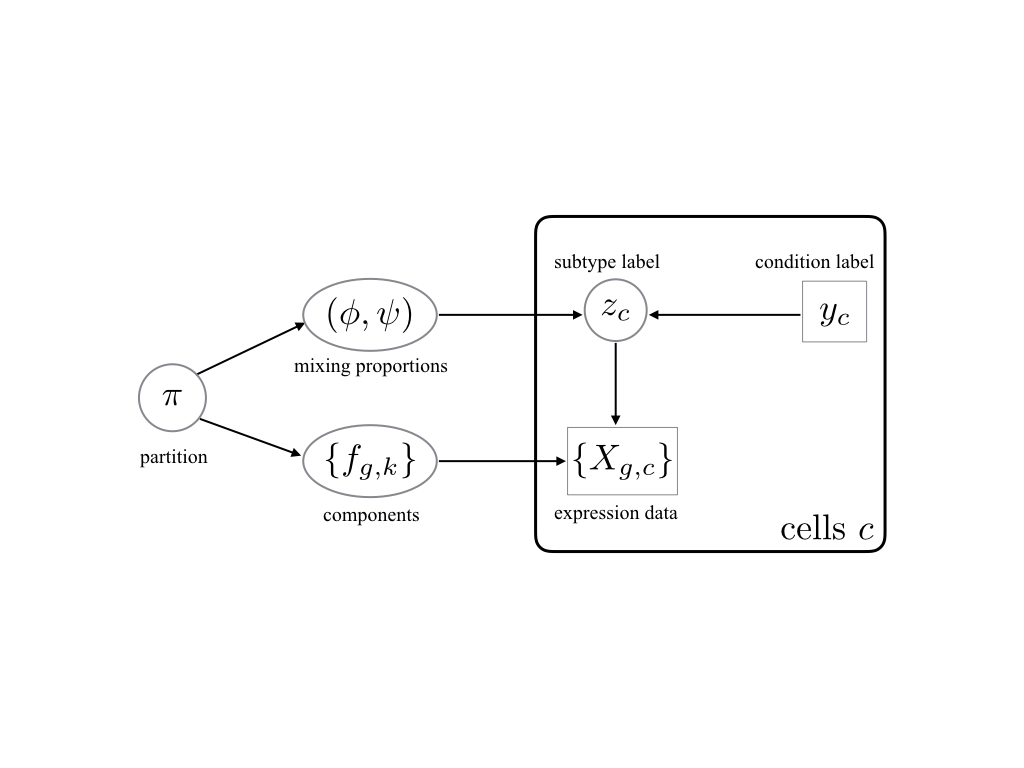
\includegraphics[trim={4cm 6cm 4cm 6cm}, clip, width=5in]{Figs/dag.png}
  \caption{Directed acyclic graph structure of compositional 
model and partition-reliant prior. The plate on the right side indicates i.i.d.
copies over cells $c$, conditionally on mixing proportions and mixing components.
 Observed data are indicated in rectangles/squares, and unobserved variables
are in circles/ovals. }
  \label{fig:dag}
\end{figure}

Key to computing the gene-specific 
local false discovery rate $P(\text{ED}_g|X,y)$ is
evaluating probabilities $P\left(A_\pi \cap M_{g,\pi} |X,y \right)$.
The dependence structure (Figure~\ref{fig:dag}) implies a useful reduction of this
quantity, at least conditionally upon subtype labels $z=(z_c)$. For each 
subtype partition $\pi$ and gene $g$,

\begin{theorem}  
 $P\left(A_\pi \cap M_{g,\pi} |X,y,z \right) 
  =  P\left(A_\pi |y,z \right) 
                      P\left(M_{g,\pi}| X,z \right)$.
\end{theorem}

In what follows, we develop the  modeling and computational elements necessary  to efficiently evaluate inference summaries~(\ref{eq:lfdr}) taking advantage of 
Theorems~1 and~2.  Roughly, the methodological idea is that subtype labels $z$
have relatively low uncertainty, and may be estimated from genome-wide 
clustering of cells in the absence of condition information $y$ (up to an arbitrary label permutation). 
The modest uncertainty in $z$
we handle through a computationally efficient randomized clustering scheme.
 Theorem~2 indicates that our computational task then separates into
two parts given $z$.  On one hand, cell subtype frequencies 
combine with condition labels to give
$P\left(A_\pi |y,z \right)$. Then gene-level data
locally drive the posterior probabilities $P\left(M_{g,\pi}| X,z \right)$ that
measure differential expression between subtypes. 
Essentially, the model provides a specific form of information 
sharing between genes  that leverages the compositional structure of single-cell 
data in order to sharpen our assessments of between-condition expression changes. 


\subsection{Method structure and clustering}

We leverage the extensive research on how to cluster cells into subtypes using scRNA-seq data:
for example,  SC3~\citep{sc3}, CIDR~\citep{CIDR}, and ZIFA~\citep{ZIFA}. 
\todo{How are these methods related to the K-mediods construction used?}
We propose clustering on the full set
of profiles in a way that is blind to the condition label vector $y$, in order to have as many cells as possible
to inform the subtype structure.  We investigated several clustering schemes in numerical experiments and allow 
flexibility in this choice within the \textsc{scDDboost} software. 
Associating clusters with subtype labels $\hat z_c$  estimates
the actual subtypes $z_c$, and prepares us to use Theorems~1 and~2 in order to compute separate
posterior probabilities $P(A_\pi|y, \hat z)$ and $P(M_{g, \pi}| X, \hat z)$ that are necessary for scoring
differential distribution. The first probability concerns patterns of cell counts over subtypes in the two conditions,
and has a convenient closed form within the double-Dirichlet model (Section~2.3).
The second probability concerns patterns of changes in expected expression levels among subtypes, and this is
also conveniently computed for negative-binomial counts using \textsc{EBSeq} \citep{ref:Leng}. 
Algorithm~\ref{alg:scDDcore}
summarizes how these elements combine to get the posterior probability of differential distribution per gene,
conditional on an estimate of the subtype labels.


\begin{algorithm}
\caption{\textsc{scDDBoost-core}}\label{alg:scDDcore}
\raggedright\hspace*{\algorithmicindent} \textbf{Input}: \begin{list}{}{}
 \item \textsc{genes} by \textsc{cells} expression data matrix $X=(X_{g,c})$
 \item  cell condition labels $y=(y_c)$ 
 \item  cell subtype labels (estimated)  $\hat z=(\hat z_c)$
 \end{list}
\hspace*{\algorithmicindent} 
\textbf{Output}:  posterior probabilities of differential distribution from estimated subtypes
\begin{algorithmic}[1]
\Procedure{scDDBoost-core}{$X,y,\hat z$}
 \item  number of cell subtypes $K = \rm{length}( \rm{unique}( \hat z ) )$  
\State subtype differential expression: $\forall g,\pi$ compute  $P(M_{g,\pi} | X, \hat z)$ using \verb+EBSeq+
\State cell frequency changes: $\forall \pi$ compute  $P(A_\pi | y, \hat z)$ using Double Dirichlet model 
\State posterior probability: $\forall g,  \, P(\text{ED}_g | X, y, \hat z)\gets \underset{\pi}{\sum}P(M_{g,\pi} | X, \hat z) \,
 P(A_\pi | y, \hat z)$
\State \textbf{return} $\forall g, \, P(\text{DD}_g |X, y, \hat z)=1-P(\text{ED}_g| X,y, \hat z)$
\EndProcedure
\end{algorithmic}
\end{algorithm}


We invoke $K-$medoids \citep{kmedoids} 
as the default clustering method in \textsc{scDDboost}, and customize the cell-cell distance by integrating two measures.  
\todo{is K-mediods used over SC3/CIDR/ZIFA because it's easier to carry out randomized clusterings? Or why?}
The first assembles gene-level information by cluster-based-similarity partitioning~\citep{ref:cspa}.
 Separately at each gene,   modal clustering (\cite{ref:dahl} and Supplementary Material Section~2.2.2) partitions the cells, and
then we define dissimilarity between cells as the Manhattan distance of those gene specific partition labels.
A second measure defines dissimilarity by one minus the 
Pearson correlation between cells, which is computationally inexpensive,
less sensitive to outliers than Euclidean distance, and effective at detecting cellular clusters in 
scRNA-seq~\citep{Cor}.
 For the default clustering in~\verb+scDDboost+, we combine these 
two measures by a weighted average, 
with  $w_C = \frac{\sigma_P}{\sigma_C + \sigma_P}$ and $w_P = 1 - w_C$. where $w_C,\sigma_C, w_P, \sigma_P$ are the weights and standard deviations of cluster-based distance and Pearson-correlation distance, respectively.  The software allows 
other distances; in any case 
the final distance matrix is denoted $D=\left( d_{i,j} \right)$. 

Any clustering method  entails classification errors, and so $\hat z_c \neq z_c$ for some cells. To mitigate
the effects of this uncertainty, \textsc{scDDboost} averages output probabilities from \textsc{scDDboost-core} over
randomized clusterings $\hat z^*$.  These are not uniformly random, but rather are generated by applying $K-$medoids
to a randomized distance matrix $D^*=\left( d_{i,j}/ w_{i,j}\right)$, 
where $w_{i,j}$ are   non-negative weights
$w_{i,j} = ( e_i + e_j )$, and where $( e_i) $ are independent and identically 
Gamma distributed deviates with shape $\hat a/2$  and rate $\hat a$, 
and where $\hat a$ is estimated from $D$. (Thus $w_{i,j}$ is Gamma$(\hat a, \hat a)$ and has unit mean.)  
The distribution of
clusterings induced by this simple computational 
scheme approximates a Bayesian posterior analysis, as we argue in
the Appendix, where we also present pseudo-code for the resulting \textsc{scDDboost} 
Algorithm~\ref{alg:scDDboost}.
Averaging over results from randomized clusterings 
 gives additional stability to the posterior probability statistics
 (Supplementary Figure S10).


Computations become more intensive the larger is the number $K$ of cell subtypes. Version 1.0 of 
\verb+scDDboost+ is restricted to $K\leq 9$, and we consider further computational
strategies in Section~5. Inferentially, 
 taking $K$ to be too large may inflate the false positive rate (Supplementary Figure S11).
 The approach
taken in \verb+scDDboost+ is to set $K$ using the validity score~\citep{selK}, which measures 
changes in within-cluster sum of squares as we increase $K$.  Our specific implementation is in
Supplementary Material Section 2.2.4.


\subsection{$P(A_\pi|y,z)$}


%** ON THE PRIOR INDEPENDENCE**
%This expresses the idea that  subtype proportions $(\phi,\psi)$ are
%uninformative about the mean expression levels   $\{\mu_{g,i}\}$). Under this assumption:
%**

We introduce the Double Dirichlet Mixture (DDM), 
which is the partition-reliant prior $p(\phi,\psi)$ indicated in~Figure~\ref{fig:dag}, 
in order to derive an explicit
formula for $P(A_\pi|y,z)$.   We lose no generality here by defining
$A_\pi = \{ (\phi,\psi): \Phi_b = \Psi_b \;  \forall b \in \pi \}$, rather than as a subset of the full
parameter space as in~(\ref{eq:asets}).   Each $A_\pi$ is closed and convex subset of the product space
holding all possible pairs of length-$K$ probability vectors.

We propose a spike-slab-style mixture prior with the following form:
\begin{eqnarray}
\label{eq:ddmix}
p(\phi,\psi) = \sum_{\pi \in \Pi} \omega_\pi  \, p_\pi(\phi,\psi ).
\end{eqnarray} 
Each mixture component $p_\pi(\phi,\psi)$ has support $A_\pi$;  
the mixing proportions $\omega_\pi$ are positive constants summing to one. 
To specify component $p_\pi$,  notice that on $A_\pi$ there is a 1-1 correspondence between pairs $(\phi, \psi)$ and 
parameter states:
\begin{eqnarray}
\label{eq:onetoone}
 \left\{ (\tilde \phi_b, \tilde \psi_b, \Phi_b), \; \forall b \in \pi \right\}, 
\end{eqnarray}
where
\begin{eqnarray*}
\tilde{\phi}_b = \frac{\phi_b}{\Phi_b}, \quad \tilde{\psi}_b = \frac{\psi_b}{\Psi_b}, \quad 
{\mbox {\rm and}} \quad \Phi_b = \sum_{k \in b} \phi_k = \sum_{k \in b} \psi_k = \Psi_b.
\end{eqnarray*}
For example, $\tilde{\phi}_b$ is a vector of conditional probabilities for each subtype given that a cell
from the first condition is one of the subtypes in $b$. 


We introduce hyperparameters
$\alpha^1_k, \alpha^2_k>0$ for each subtype $k$, and set 
$\beta_b = \sum_{k \in b}\left( \alpha^1_k + \alpha^2_k \right)$ for any possible block $b$.
Extending notation, let $\alpha_b^j$ be the vector of $\alpha_k^j$
for $k\in b$, $\beta_\pi$ be the vector of $\beta_b$ for $b \in \pi$, $\phi_b$ and $\psi_b$ be vectors
of $\phi_k$ and $\psi_k$, respectively, for $k\in b$, and $\Phi_\pi$ and $\Psi_\pi$ be the vectors
of $\Phi_b$ and $\Psi_b$ for $b \in \pi$.  The proposed double-Dirichlet component 
$p_\pi$ is determined in the transformed scale by assuming $\Psi_\pi = \Phi_\pi$ and further:
\begin{eqnarray}
\label{eq:doubledir}
\Phi_\pi  &\sim& \text{Dirichet}_{N(\pi)}[   \beta_\pi   ]  \\ \nonumber
\tilde \phi_b  &\sim & \text{Dirichlet}_{N(b)}[ \alpha_b^1 ] \qquad \forall b \in \pi \\ \nonumber
\tilde \psi_b  &\sim & \text{Dirichlet}_{N(b)}[ \alpha_b^2 ] \qquad \forall b \in \pi 
\end{eqnarray}
where $N(\pi)$ is the number of blocks in $\pi$ and $N(b)$ is the number of subtypes in $b$, and
where all random vectors in~(\ref{eq:doubledir}) are mutually independent.  
Mixing over $\pi$ as in~(\ref{eq:ddmix}), we write
$(\phi,\psi) \sim {\mbox {\rm DDM}}\left[ \omega=(\omega_\pi),
\alpha^1=(\alpha^1_k), \alpha^2 = (\alpha^2_k) \right].$


We record some properties of the component distributions $p_\pi$:
%%using the well-known Dirichlet-multinomial conjugacy and the Dirichlet collapsing property~\citep{ref:Dickey}. 

\noindent
{\bf Property 1:}  In $p_\pi(\phi,\psi)$, $\psi$ and $\phi$ are dependent, unless $\pi$ is the null 
partition in which all subtypes constitute a single block.

%\noindent
%{\bf Property 2:}  If $\alpha^1=\alpha^2$, then both $\phi$ and $\psi$ are marginally distributed
%as Dirichlet$_K(\alpha^1)$.  

\noindent
{\bf Property 2:} With $k \in b$, marginal means are:
\begin{eqnarray*}
E_\pi\left( \phi_k \right ) = \frac{ \alpha^1_k }{ \sum_{k' \in b} \alpha^1_{k'} } \,
		\frac{ \beta_b }{ \sum_{b' \in \pi} \beta_{b'} } \quad {\mbox {\rm and}} \quad
E_\pi\left( \psi_k \right ) = \frac{ \alpha^2_k }{ \sum_{k' \in b} \alpha^2_{k'} }  \,
		\frac{ \beta_b }{ \sum_{b' \in \pi} \beta_{b'} } .
\end{eqnarray*}

Recall from~(\ref{eq:counts}) the vectors $t^1$ and $t^2$ holding
counts  of cells in each subtype in each condition, computed from $y$ and $z$.  Relative to a block $b \in \pi$, 
let $t^j_b = \sum_{k\in b} t^j_k$, for cell conditions $j=1,2$, and,
let $t^j_\pi$ be the vector of these counts over $b \in \pi$.   The following properties refer to
marginal distributions in which $(\phi,\psi)$ have been integrated out of the joint
distribution involving~(\ref{eq:mult}) and the component $p_\pi$.

\noindent
{\bf Property 3:}  $t^1$ and $t^2$ are conditionally independent given $y$, $t^1_\pi$ and $t^2_\pi$.

\noindent
{\bf Property 4:}  For $j=1,2$,
\begin{eqnarray*}
p_\pi(t^j | t^j_{\pi},y) = \prod_{b \in \pi} \left\{
\left[ \frac{ \Gamma(t^j_b +1 ) }{\prod_{k \in b} \Gamma( t^j_k + 1 ) } 
\right]
\left[ \frac{\Gamma( \sum_{k \in b} \alpha_k^j )}{
		\prod_{k\in b} \Gamma( \alpha_k^j ) } \right] 
       \left[        \frac{ \prod_{k \in b} \Gamma(\alpha_k^j + t^j_k)  }{
		\Gamma(t^j_b + \sum_{k\in b} \alpha_k^j ) )}\right]
 \right\}
\end{eqnarray*}

\noindent
{\bf Property 5:}  
\begin{eqnarray*}
p_\pi(t^1_{\pi},t^2_{\pi}| y) =
 \left[ \frac{ \Gamma(n_1+1) \Gamma(n_2+1) }{ \prod_{b \in \pi} \Gamma(t^1_b+1) 
   \Gamma( t^2_b + 1 )} \right] 
\left[ \frac{\Gamma( \sum_{b \in \pi} \beta_b  )}{
   \prod_{b \in \pi} \Gamma(\beta_b )} \right] 
 \left[ \frac{ \prod_{b \in \pi} \Gamma( \beta_b + t^1_b + t^2_b )}{
	\Gamma( n_1 + n_2 + \sum_{b \in \pi} \beta_b  )} \right].
\end{eqnarray*}


Let's look at some special cases to dissect this result. 

Case 1. If $\pi$ has a single block equal to the entire
 set of cell types $\{1,2, \cdots, K\}$,  then $t^j_b=n_j$ for both $j=1,2$,
and Property~5 reduces, correctly, to 
$p_\pi(t^1_{\pi},t^2_{\pi}| y) = 1$.  Further,
\begin{eqnarray*}
p_\pi(t^j | t^j_{\pi},y) = 
\left[ \frac{ \Gamma(n_j +1 ) }{ \Gamma( n_j + \sum_{k=1}^K \alpha_k^j ) }
\right]
\left[ \frac{\Gamma( \sum_{k =1}^K \alpha_k^j )}{
                \prod_{k=1}^K \Gamma( \alpha_k^j ) } \right]
       \left[    \prod_{k=1}^K    \frac{  \Gamma(\alpha_k^j + t^j_k)}{
                \Gamma(t^j_k + 1 )}\right]
\end{eqnarray*}
which is the well-known Dirichlet-multinomial predictive distribution
for counts $t^j$~\citep{Wag}.  E.g, taking $\alpha_k^j=1$ for all types $k$ 
we get the uniform distribution
\begin{eqnarray*}
p_\pi(t^j | t^j_{\pi},y) = 
 \frac{ \Gamma(n_j +1 ) \Gamma(K) }{ \Gamma( n_j + K ) }.
\end{eqnarray*}

Case 2. At the opposite extreme, $\pi$  has one block $b$ for each
 class $k$, so $\phi=\psi$. Then $p_\pi(t^j | t^j_{\pi},y) = 1$, and 
further, writing $b = k$,
\begin{eqnarray*}
p_\pi(t^1_{\pi},t^2_{\pi}|y ) =
 \left[ \frac{ \Gamma(n_1+1) \Gamma(n_2+1) }{ \prod_{k=1}^K 
   \Gamma(t^1_k+1) 
   \Gamma( t^2_k + 1 )} \right] 
\left[ \frac{\Gamma( \sum_{k=1}^K \beta_k  )}{
   \prod_{k=1}^K \Gamma(\beta_k)} \right] 
 \left[ \frac{ \prod_{k=1}^K \Gamma( \beta_k + t^1_k + t^2_k )}{
	\Gamma( n_1 + n_2 + \beta_k  )} \right].
\end{eqnarray*}
which corresponds to Dirichlet-multinomial predictive distribution for counts $t^1 + t^2$ 
since $t^1$ and $t^2$ are identical distributed given $(\phi,\psi)$ in this case.  These properties 
are useful in establishing:
\begin{theorem}
DDM is conjugate to multinomial sampling of $t^1$ and $t^2$:
\begin{eqnarray*}
(\phi,\psi)|y,z  \sim {\mbox {\rm DDM}}\left[ \omega^{\rm post}=(\omega^{\rm post}_\pi), \alpha^1 + t^1, \alpha^2 + t^2  \right]
\end{eqnarray*}
where
\begin{eqnarray}
\label{eq:postmix}
\omega^{\rm post}_\pi \propto 
 p_\pi(t^1 | t^1_{\pi},y)\, p_\pi(t^2|  t^2_{\pi},y )
 \, p_\pi( t^1_{\pi}, t^2_{\pi} | y ) \, \omega_\pi.
\end{eqnarray}

\end{theorem}


The target probability $P(A_\pi|y,z)$ is an integral of the posterior distribution in Theorem~3.
To evaluate it, we need to contend with the fact that sets $\{ A_\pi: \pi \in \Pi \}$ are not disjoint.
Relevant overlaps have to do with partition refinement.  Recall 
that a  partition $\pi^r$ is a refinement of a partition $\pi^c$ if for any $b \in \pi^c$ there 
exists $s \subset \pi^r$  such that $\underset{b'\in s}\cup b' = b$. 
We say $\pi^c$  coarsens $\pi^r$ when $\pi^r$ refines $\pi^c$. Any partition both
refines and coarsens itself, as a trivial case. 
Generally, refinements increase the number of blocks.
 If subtype frequency vectors $(\phi,\psi)$
satisfy the constraints in $A_{\pi^r}$ then they also satisfy the constraints of any $\pi^c$
that coarsens $\pi^r$: i.e., $A_{\pi^r} \subset A_{\pi^c}$.  
Refinements reduce the dimension of allowable parameter states. 
% and the mixture structure of DDM gives positive probability  (spikes) on such subsets.  
 For the double-Dirichlet
component distributions $P_\pi$, we find:

\noindent
{\bf Property 6:} For two partitions $\tilde \pi$ and $\pi$,  
$P_{\tilde \pi}\left( A_{\pi} | y,z \right) = 1[ {\mbox {\rm $\tilde \pi$ refines $\pi$ }}].$

This supports the main finding of this section:
\begin{eqnarray}
\label{eq:mainfinding}
P(A_\pi|y,z) = 
\sum_{\tilde \pi \in \Pi} \omega^{\rm post}_{\tilde \pi} \,  1[ {\mbox {\rm $\tilde \pi$ refines $\pi$}} ].
\end{eqnarray}


\subsection{$P(M_{g,\pi}|X,z)$}
We leverage well-established modeling techniques for transcript analysis, including
\cite{ref:Leng}, \cite{Kendziorski:2003aa}, and~\cite{Jensen:2009aa}, which characterize
 equivalent or differential expression in terms of shared or independently drawn mean effects.  Let
$X_{g,b}$ denote
the subvector of expression values at gene $g$ over cells $c$ with $z_c=k$ for which subtype $k$ is part of
 block $b$ of partition $\pi$.  Conditioning on subtype labels $z=(z_c)$,  we assume that under $M_{g, \pi}$: 
\begin{enumerate}
\item {\em between blocks:} subvectors $\{ X_{g,b}: b \in \pi \}$ are mutually independent,
\item {\em within blocks:} for cells mapping to block $b$, observations $X_{g,c}$ are i.i.d. 
\item {\em mean effects:}  for each block $b$, there is a univariate mean, say $\mu_{g,b}$, 
 shared by cells mapping to that block.  {\em a priori} these means are i.i.d.  between blocks.
\end{enumerate}
These assumptions imply a useful factorization marginally to latent means,
\begin{eqnarray}
\label{eq:ebseq}
P(X_g|M_{g,\pi}, z) = \prod_{b \in \pi} f(X_{g,b}),
\end{eqnarray}
where $f$ is a customized density kernel.  In our case we use \verb+EBseq+ from~\cite{ref:Leng}: 
the sampling distribution of
 $X_{g,c}$ is negative binomial, and $f$ becomes a particular compound multivariate 
negative binomial formed from integrating
uncertainty in the block-specific means (see Supplementary Material Section 2.2.1).  
Through its gene-level mixing model,
\verb+EBseq+ also gives estimates of $\{ P(M_{g,\pi}|z) \}$: the proportions of genes governed by any of the 
different patterns $\pi$ of equivalent/differential expression among subtypes. With these estimates 
and~(\ref{eq:ebseq}) we compute by Bayes' rule:
\begin{eqnarray*}
P(M_{g,\pi}|X,z) \propto P(M_{g,\pi}|z) \, \prod_{b \in \pi} f(X_{g,b}).
\end{eqnarray*}
The proportionality is resolved by calculating over all partitions $\pi$.

 
\section{Numerical experiments}
\todo{What I don't get a sense from the sims is how it scales with n}

\subsection{Synthetic data} 
We used \verb+splatter+ (v. 1.2.0)  
to generate synthetic scRNA-seq  data for which the DD status of genes is known~\citep{ref:Zappia}, 
 thereby allowing us to 
measure operating characteristics of \verb+scDDboost+.  Our hypothetical two-condition comparison involved
17421 genes, 10\% of which exhibited actual shifts in distribution between the two conditions. 
We entertained 12 different parameter settings encoding these distributional shifts, 
varying the number of subtypes $K$, the subtype frequency profiles $(\phi,\psi)$, as well
as the  \verb+splatter+-specific parameters $\theta$ and $\gamma$ controlling location and scale characteristics
of expression levels. These settings cover a range
of scenarios we might expect to see in practice.  Two replicate data sets were simulated under each parameter setting.
Further details are in Supplementary Material Section~3.1.   

Figures~\ref{fig:sim1} and~\ref{fig:sim2} summarize the true positive rate and false discovery rate
of \verb+scDDboost+ compared to three other methodologies: \verb+MAST+ (v. 1.4.0), \verb+scDD+ (v. 1.2.0), and 
\verb+DESeq2+ (v. 1.18.1). 
\verb+scDDboost+ exhibits very good operating characteristics in this study, as it controls the 
FDR in all cases while also delivering a relatively high rate of true positives in all cases.


\begin{figure}[H]
  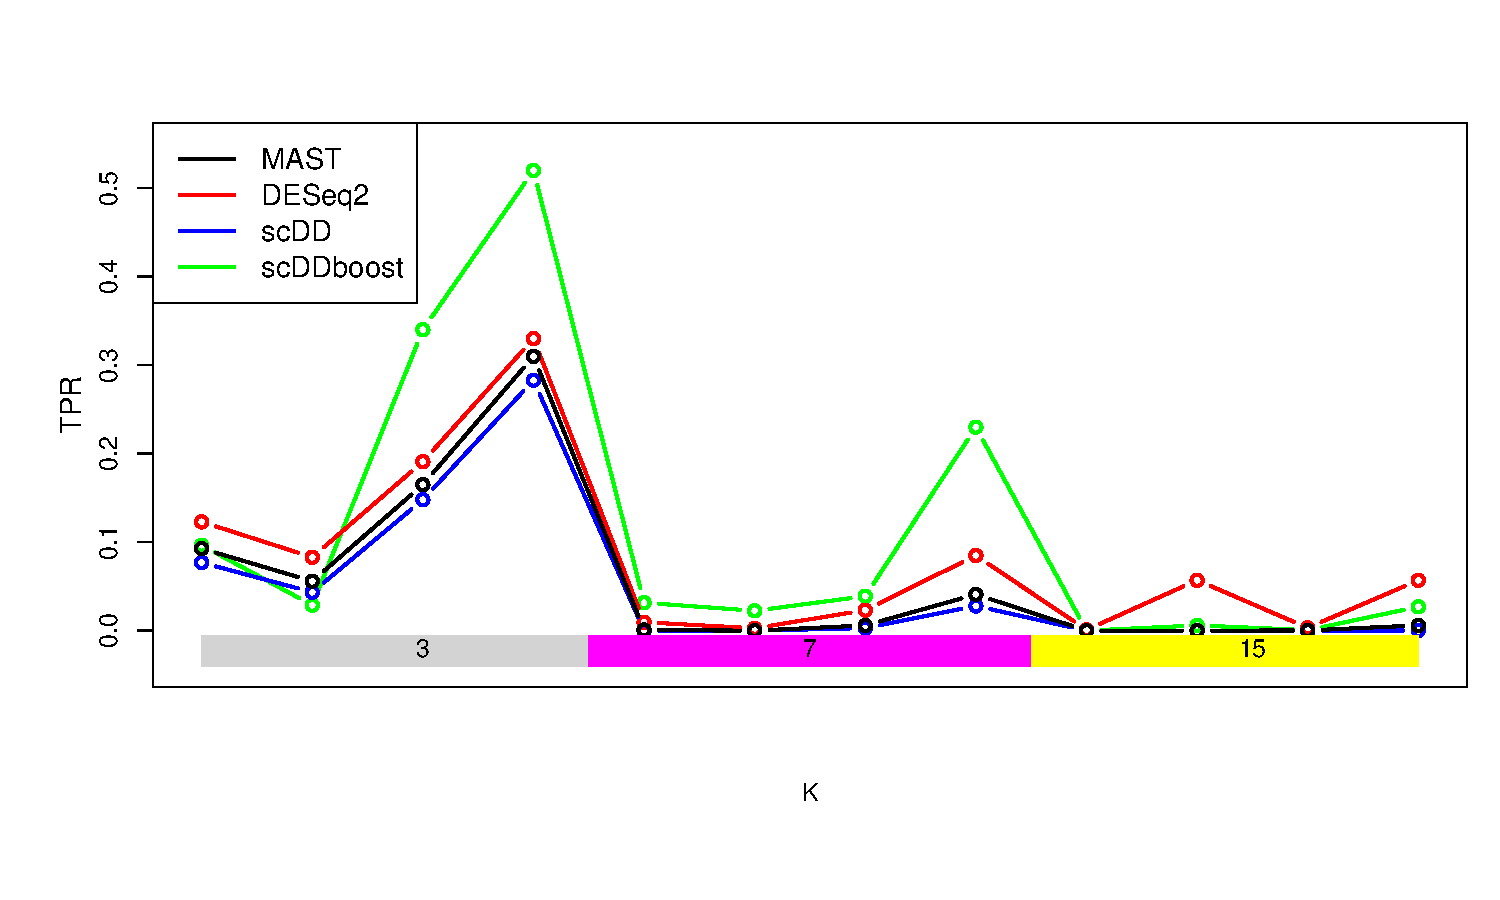
\includegraphics[width = 0.95\textwidth]{Figs/simuTPR.pdf}
  \caption{True positive rate (vertical) of four DD detection methods in 12 synthetic-data settings (horizontal). 
  Settings are labeled for $K / \theta / \gamma$  and ranked by scDDboost values. Each method
 is targeting a 5\% false discovery rate (FDR). The plot shows  average rates over replicate simulated data
 in each setting.
   }
  \label{fig:sim1}
\end{figure}


\begin{figure}[H]
  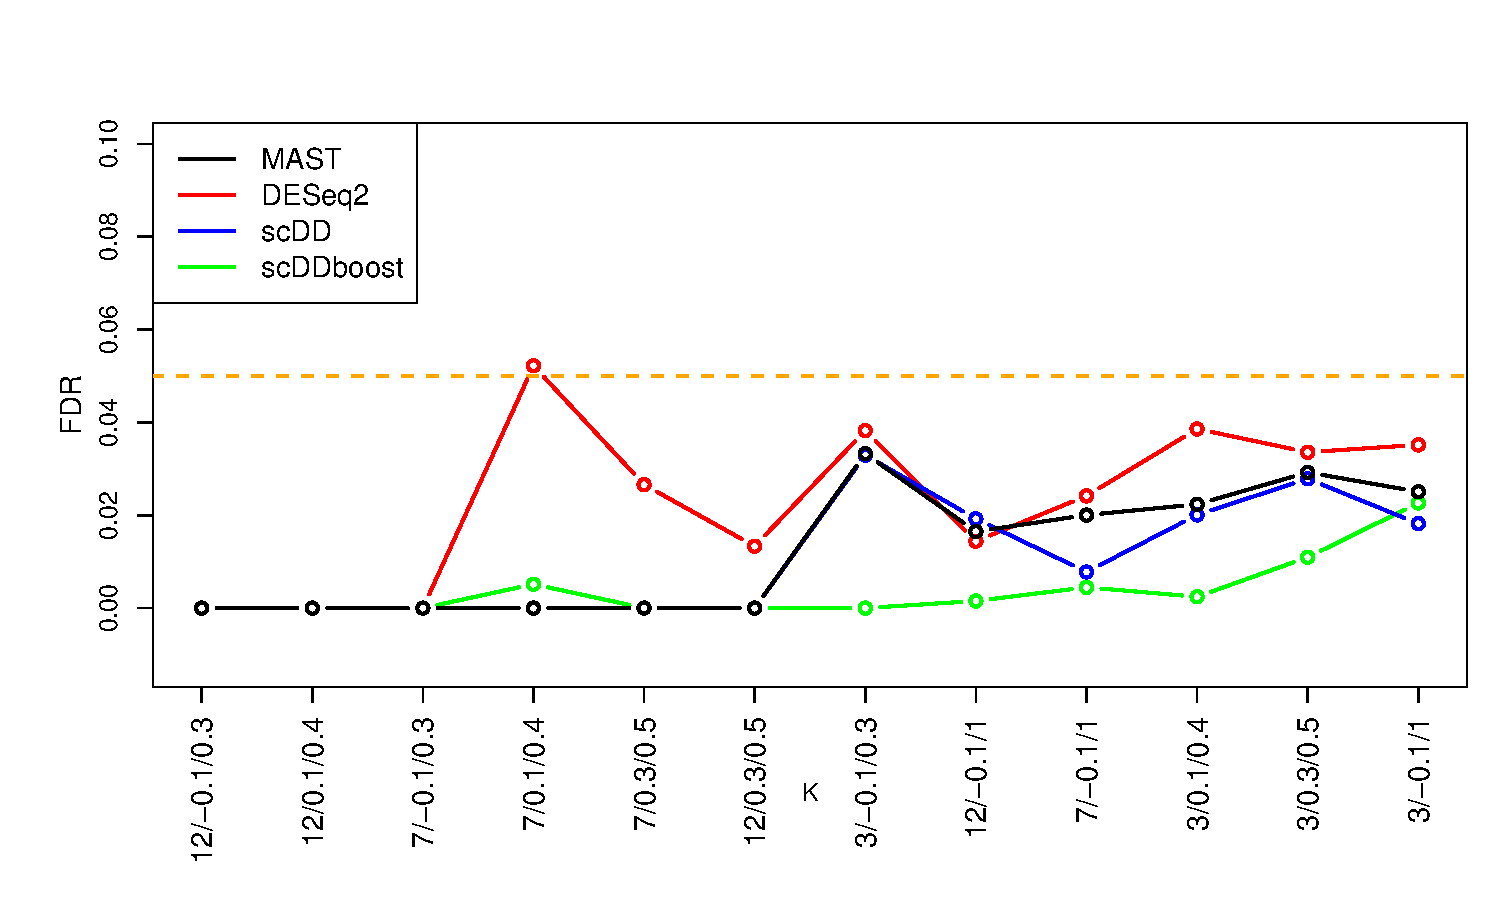
\includegraphics[width = 0.95\textwidth]{Figs/simuFDR.pdf}
  \caption{False discovery rate (vertical) of methods in settings (horizontal, same order) from Figure~\ref{fig:sim1} }
  \label{fig:sim2}
\end{figure}


\subsection{Empirical study}

We applied \verb+scDDboost+ to a collection of previously published
data sets that are recorded at \verb+conquer+~\citep{ref:Cq}.  
\todo{All are non-UMI protocols, correct? Curious to see performance on
a UMI dataset, as they present further challenges}
Though not knowing the truly DD
genes, we can examine how \verb+scDDboost+ output compares to output from some standard methods.  We selected
12 data sets from \verb+conquer+   representing different species and experimental settings
and involving hundreds to thousands of cells.   Appendix Table \ref{table:1} provides details.  Figure~\ref{fig:es} compares
methods in terms of the size of the reported list of DD genes at the 5\% FDR target level.  
We see a consistently high yield of \verb+scDDboost+ among the evaluated  methods.  For reference, one of these data 
sets (GSE64016) happens to be the data behind Figure~\ref{fig:whet}, where we know from other information that some
of the uniquely identified genes are likely not to be false positives.


\begin{figure}[H]
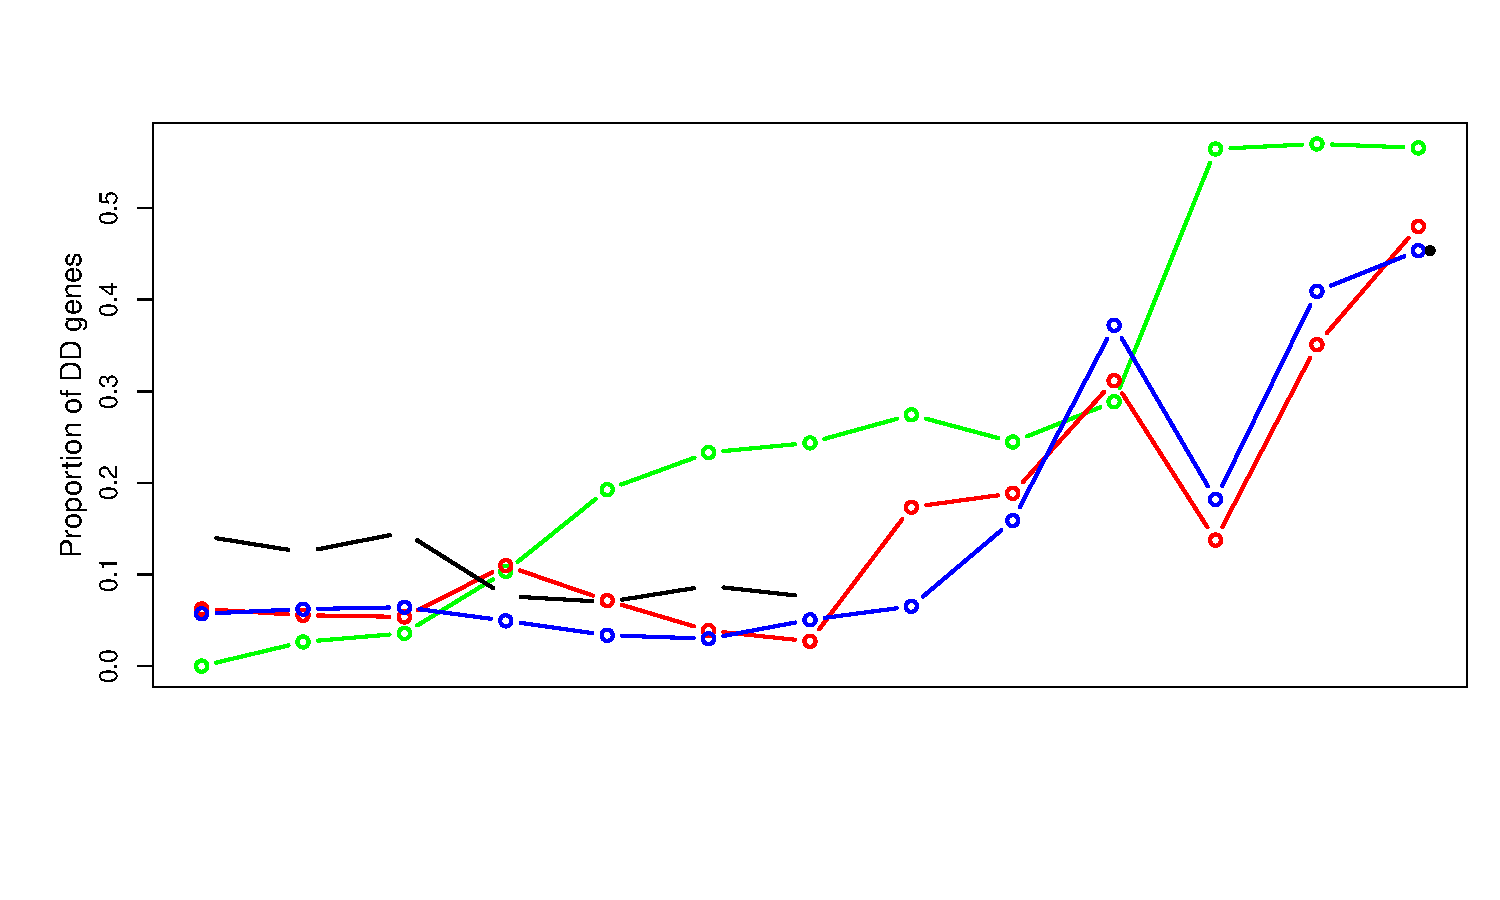
\includegraphics[width = 0.95\textwidth]{Figs/DD95.pdf}
 \caption{Proportion of DD genes at 5\% FDR threshold with respect to total number of genes identified by each method. Ranked by 
 scDDboost list size }
  \label{fig:es}
\end{figure}


To check that the increased discovery rate
of   \verb+scDDboost+ is  not associated with an increased rate of false calls, we 
applied it to a series of random splits of single-condition data sets (Appendix Table \ref{table:2}). Figure~\ref{nullperm}
confirms a very low call rate in cases where no changes in distribution are expected.



\begin{figure}[H]
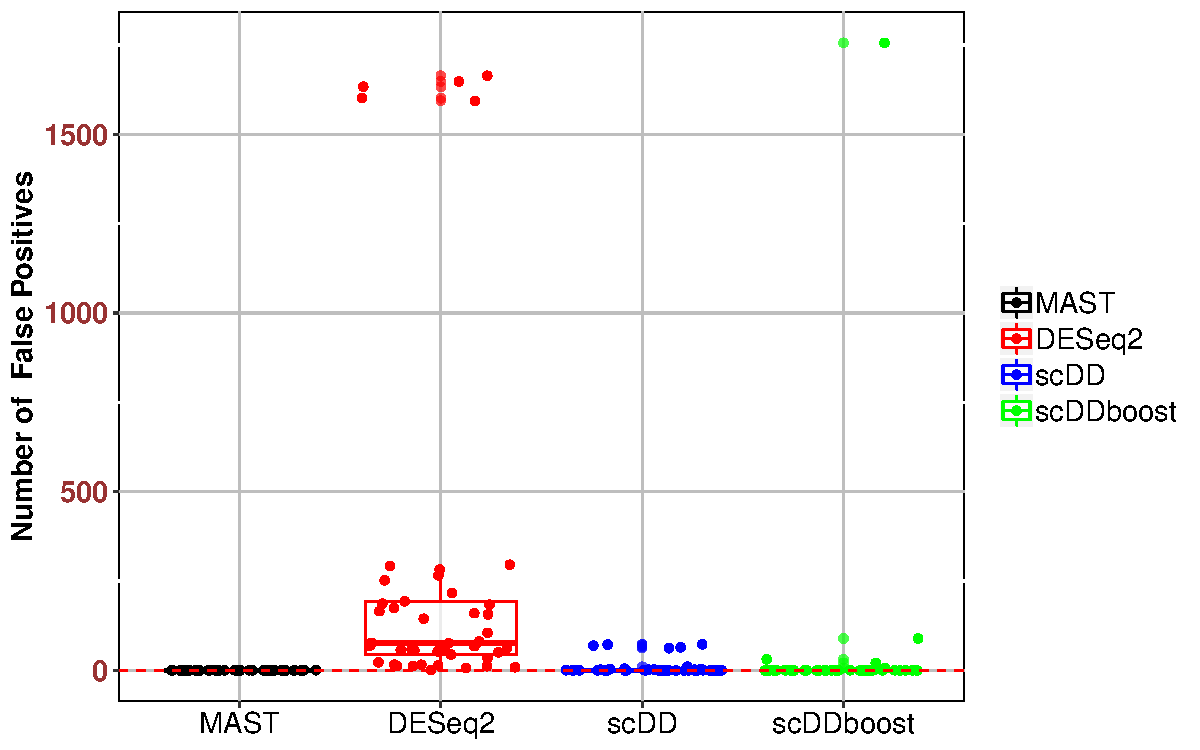
\includegraphics[width = 0.8\textwidth]{Figs/fdrCounts.pdf}
 \caption{False positive counts at 5\% FDR threshold by several methods on  5 random splits of 9 single-condition
data sets from Appendix Table \ref{table:2}} \label{nullperm}
\end{figure}


We conjecture that \verb+scDDboost+ gains power through its novel approach to borrowing strength across genes;
i.e., that the genomic data are providing information about cell subtypes and mixing proportions,
leaving gene-level data to guide gene-specific mixture components. One way to drill into this
idea is to consider how many genes have similar expression characteristics to a given gene on
test.
\todo{Not sure what is meant by 'on test'} 
By virtue of the \verb+EBseq+ analysis inside \verb+scDDboost+, we may assign each gene to
a set that all have the same highest-probability pattern of equality/inequality of means across
the subtypes. Say $\hat \pi_g = {\rm argmax}_{\pi} P( M_{g,\pi} | \hat z, X)$. 
In Figure~\ref{fig:shift}, we show
that compared to DD genes commonly identified by multiple methods (blue), the set sizes for genes
uniquely identified by \verb+scDDboost+ (red) tend to be larger.  Essentially, the proposed methodology
 boosts weak DD evidence when a gene's pattern of differential expression among cell subtypes
matches a large number of other genes. 


\begin{figure}[H]
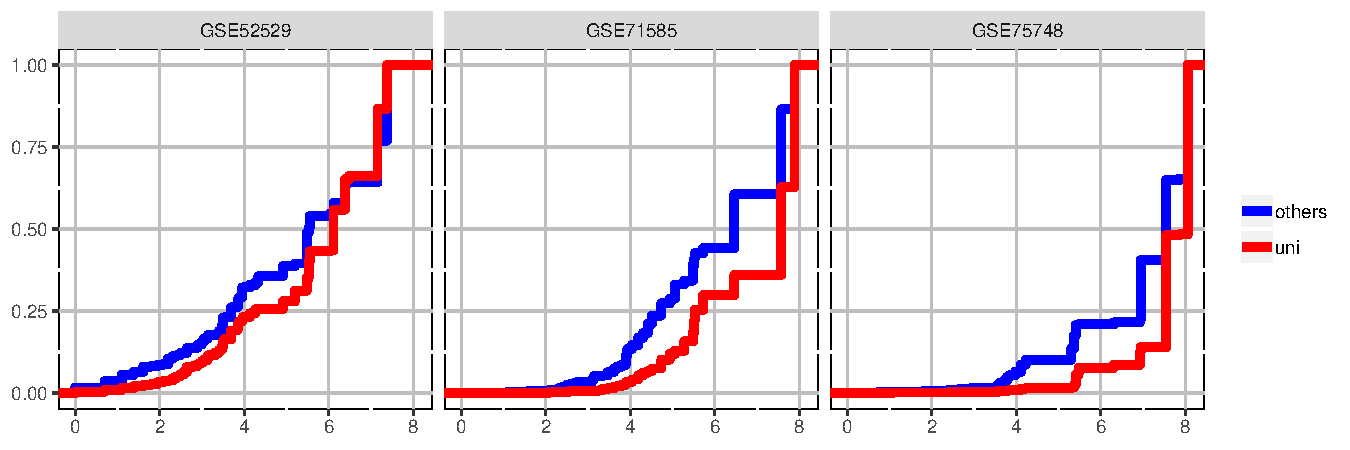
\includegraphics[width = 0.9\textwidth]{Figs/shift.pdf}
 \caption{
 Genes are grouped by their pattern of differential expression across subtypes as inferred by
the EBseq computation within scDDboost for three example datasets.
 Cumulative distribution
functions of the log-scale size statistic for all genes 
 identified by scDDboost are plotted; red is the subset uniquely identified by scDDboost; blue are those also identifed by the comparison methods (MAST, scDD, or DESeq2).
 Sets of similarly-patterned genes tend to be larger (horizontal axis, log size) for genes uniquely
 identified by scDDboost (red) compared to other DD genes (blue), at 5\% FDR.}
  \label{fig:shift}
\end{figure}
\todo{axes labels missing in fig 8}
% Datasets used for demonstration from left to right are GSE71585, GSE64016, EMTAB2805.



%\begin{figure}[H]
%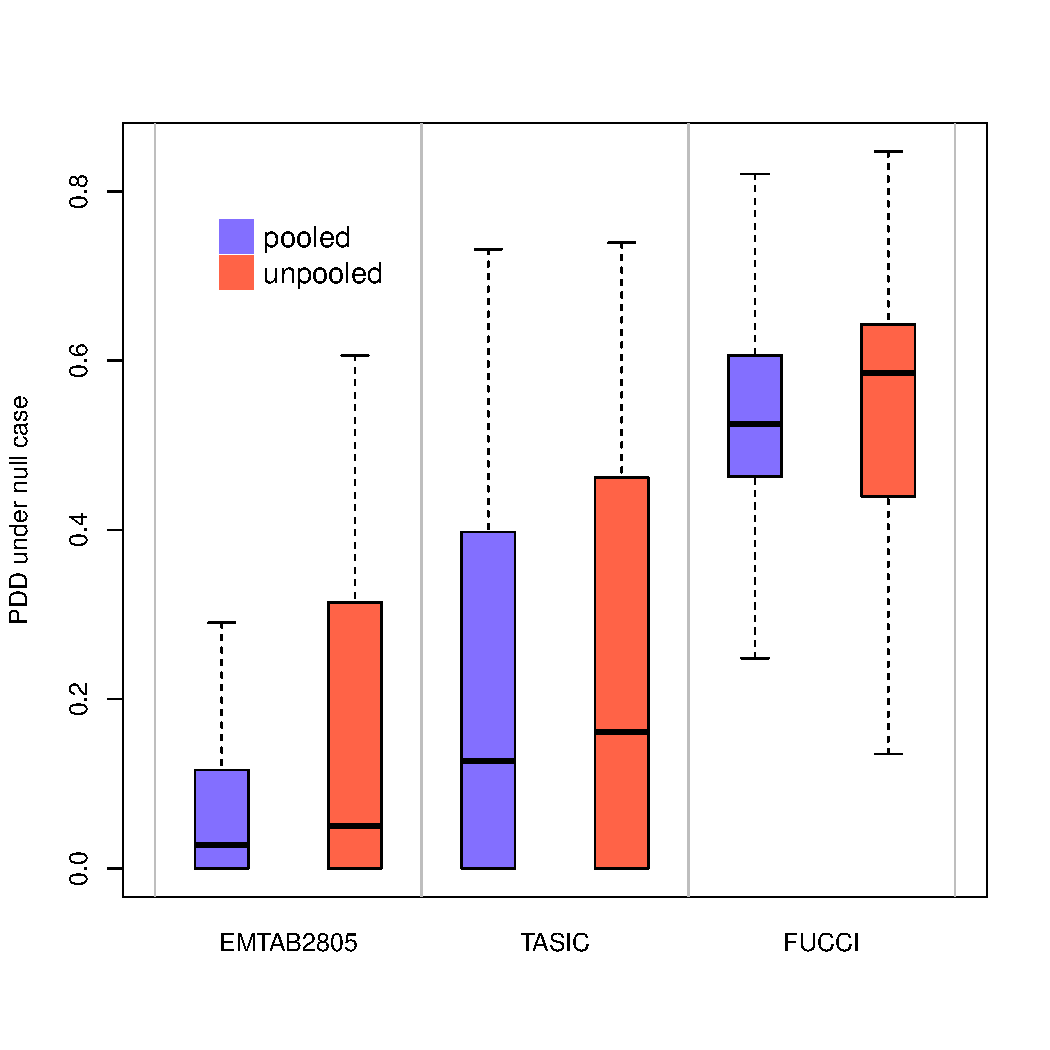
\includegraphics[width = 0.7\textwidth]{Figs/nullpdd_box.pdf}
% \caption{PDD of the same datasets used in Figure 7, we have types of PDD, the purple box is the PDD calculated by using the proportion of DE patterns inferred from the whole genome.  
% The magenta box is the PDD using the trivial proportion of DE pattern (i.e. all DE patterns between subtypes have same probabilities), basically we do not borrow information from other genes. 
% In the null case, we observed lower PDD when using information from the whole genome and this is consistent with the underlying ED structure. 
% Recall in Figure 7, genes uniquely identified by scDDboost tend to associate with DE pattern with large size. From the null case such behavior could make our PDD more correct}
%  \label{fig:EBSeq}
%\end{figure}
%**{\em Xiuyu, please improve the figure on PDD and put into Supplementary.  We can put some summary sentences
%here if they fit well. The point may go better in the discussion section.} **





\subsection{Bursting}


Transcriptional bursting is a fundamental property of genes. In its simplest form, the gene exists in two states: one where activity is negligible and one where there is a certain probability of 
activation~\citep{Raj:2008aa}. 
D3E~\citep{ref:d3e} is a computationally intensive 
method for DE gene analysis rooted in modeling the bursting process. It 
considers transcripts as in the stationary distribution from an 
experimentally validated stochastic process of single-cell gene expression \citep{Peccoud:1995aa}. 
Three mechanistic parameters (rate of promoter activation, rate of promoter inactivation, 
 and the conditional rate of transcription given an active  promoter) characterize the model, which allow
 distributional changes between conditions without changing the mean expression level.
For genes identified as DD by \verb+scDDboost+ in dataset GSE71585, either uniquely or in common with
comparison methods, Figure~\ref{fig:bursting} shows  changes of these bursting parameters. Interestingly, 
 genes uniquely identified by \verb+scDDboost+ are associated with more 
significant changes between estimated bursting parameters compared to commonly identified genes.
This finding and similar findings on other data sets (not shown) provide some evidence that \verb+scDDboost+
is able to detect biologically meaningful changes in the expression distribution.
\todo{how many points are in each boxplotin figure 9? }


\begin{figure}[H]
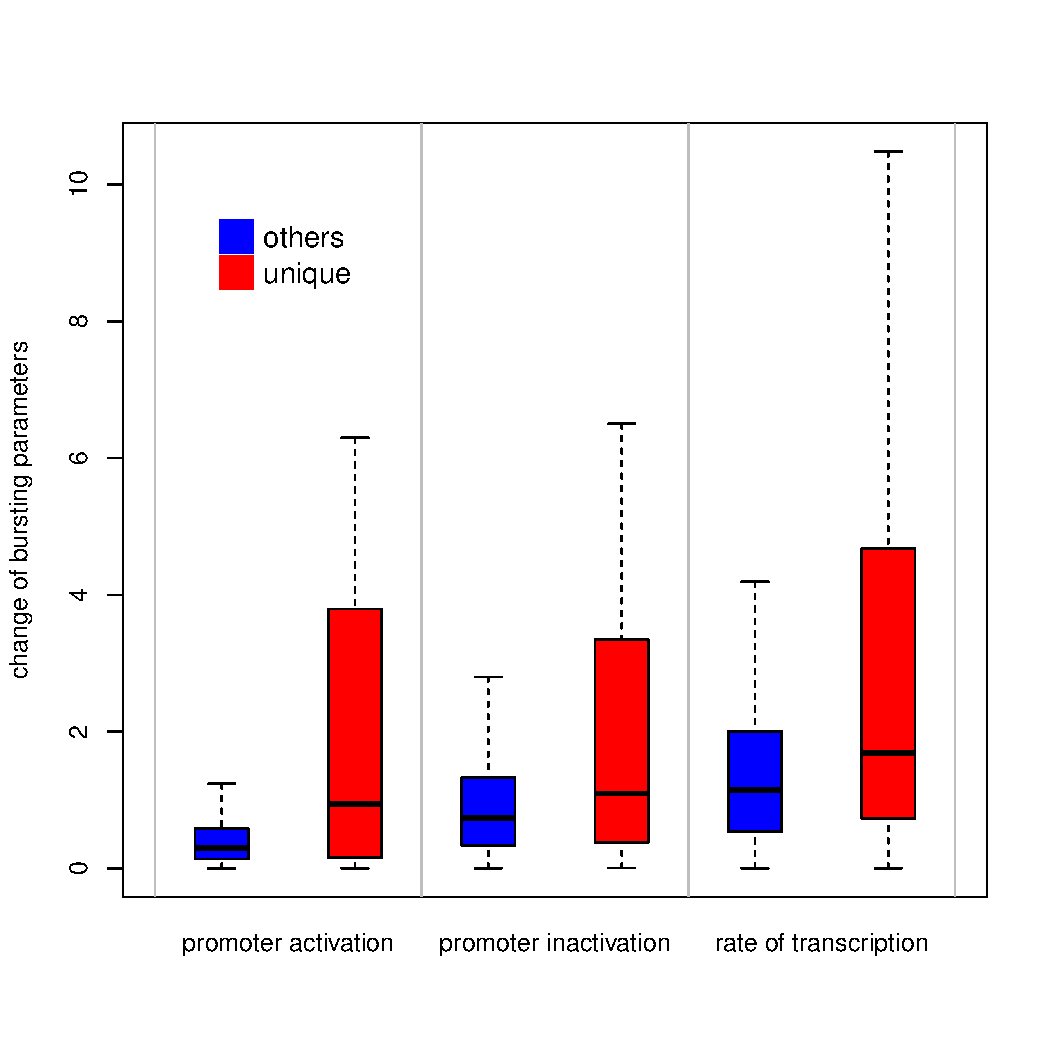
\includegraphics[width = 0.85\textwidth]{Figs/D3E_box.pdf}
\caption{ Absolute values of log fold changes of bursting parameters tend to be larger for 1758 genes uniquely identified by scDDboost (red) compare to other 2983 genes (blue) at 5\% FDR}
 \label{fig:bursting}
\end{figure}


\subsection{Time Complexity}

Time complexity of \texttt{scDDboost} can attribute to two parts: clustering and \texttt{EBSeq}. 
Recall the notation that $n$ for number of cells, $G$ for number of genes and $K$ for number of subtypes. 
The time complexity for clustering is O($Gn^2$)( O($n^2$) for one gene, supplementary section 2.2.2).
\texttt{EBSeq} use sum of counts within each subtype (sufficient statistics) to compute density kernel and for each gene there are Bell$(K)$ DE patterns to compute, 
which yields the time complexity: O($n$) + O($G\text{Bell}(K)$). 
Where Bell($K$) is the bell number(number of ways to partition $K$ elements.) 
As $G$ is roughly O(10000) and fixed.
The scalability of \texttt{scDDboost} to large samples depends on $n$ and $K$.  
\texttt{scDDboost} can efficiently dealing with large $n$ under moderate size of $K$. 
As clustering can be parallel computed by genes and the computation cost in \textt{EBSeq} is linear with $n$. 
Currently it is a computational challenge for big $K$, we will revisit this at section 5.



\section{Asymptotics of the Double Dirichlet Mixture}
\todo{Might be informative to emphasize the practical significance of the finding}
Summary statistics $P(A_\pi|y,z)$, from Section 2.3, are amenable to a first-order asymptotic analysis
that provides further insight into DDM model behavior.  The fact that support sets $A_\pi$ for component 
distributions $p_\pi( \phi,\psi)$ are not disjoint becomes an important issue.  Consider
distinct partitions $\pi_1$ and $\pi_2$  of subtypes $\{ 1, 2, \cdots, K\}$, and recall that $N(\pi)$ counts
 the number of blocks in partition $\pi$.   In case $\pi_2$ refines $\pi_1$, then $N(\pi_1) < N(\pi_2)$,
and  we also know that 
 $A_{\pi_2} \subset A_{\pi_1}$, since refinement 
imposes additional constraints on the pair $(\phi, \psi)$ of probability vectors.   
If the data-generating state $(\phi, \psi) \in A_{\pi_2}$, one might ask how posterior probability mass
tends to be allocated among the other mixture components whose
 support sets also contain this state.     The question is addressed 
by the following:

\begin{theorem}  Let $\pi_1$ and $\pi_2$ denote two partitions for which $N(\pi_1) < N(\pi_2)$
 and $A_{\pi_1} \cap A_{\pi_2}$ is non-empty. 
 Let $(\phi,\psi) \in A_{\pi_1} \cap A_{\pi_2}$ denote the data generating state for 
subtype labels $z_1, z_2, \cdots, z_n$ given i.i.d. Bernoulli condition labels $y_1, y_2, \cdots, y_n$, 
and recall the posterior mixing proportions $\omega^{\rm post}_\pi$ from equation~(\ref{eq:postmix}) with 
hyper-parameters $\alpha_i^j \geq 1 \, {\mbox {\rm for}} \,  i = 1, \cdots, K, \, j = 1,2$.   Then
\begin{eqnarray*}
\frac{\omega^{\rm post}_{\pi_1} }{ \omega^{\rm post}_{\pi_2} } \longrightarrow_{a.s.} 0 \qquad 
 {\mbox {\rm as $n \longrightarrow \infty$}}. 
\end{eqnarray*}
\end{theorem}
Essentially, mixing mass is transferred to components associated with the most refined partition
consistent with a given parameter state.  To be precise, let $H(\phi,\psi) = \{ \pi: (\phi,\psi) \in A_{\pi} \}$
record all the partitions associated with one state.   Typically, there is a most refined partition,
say $\pi^* = \pi^*(\phi,\psi)$, such that
\begin{eqnarray}
\label{eq:notQ}
A_{\pi^*} = \bigcap_{\pi \in H(\phi,\psi)} A_\pi.
\end{eqnarray}
This always happens when $K \leq 3$.  In Supplementary Material Section~4 we characterize 
the exceptional set of states where~(\ref{eq:notQ}) does not hold.  Notably, if~(\ref{eq:notQ}) does hold for
state $(\phi,\psi)$, then for any $\pi \in H(\phi,\psi)$, using Theorem~4 and~(\ref{eq:mainfinding}), we have
\begin{eqnarray*}
P(A_\pi|y_1,\cdots,y_n; z_1, \cdots z_n ) \longrightarrow_{a.s.} 1 \quad {\mbox {\rm as $n \longrightarrow \infty$}}.
\end{eqnarray*}




\section{Concluding remarks}

We have presented \verb+scDDboost+,  a tool for
 detecting differentially distributed genes from scRNA-seq data,
where transcripts are modeled as mixture of cellular subtypes. 
The methodology links established model-based
techniques with novel empirical Bayesian 
modeling and computational elements to  provide a powerful detection method showing 
comparatively good operating characteristics in simulation, empirical, and asymptotic studies.

In the software and numerical experiments we made specific choices,
 such as to use mixtures of negative binomial components per gene, and to use K-medoids
clustering on particular cell-cell distances.   These choices have evident advantages, but the 
model structure and theory developed in Section~2 carry through for other cases. Future experiments
could study other formulations within the same schema; for example there may be cell-cell 
distances that better capture the intrinsic dimensionality of expression programs, including, perhaps
distances based on diffusions \citep{Haghverdi:2015aa} or  
the longest-leg path distance \citep{Little2017PathBasedSC}.
Further, assuming a compositional structure to drive model-based computations may not be restrictive,
since it allows great flexibility in the form of each gene/condition-specific expression distribution
(as coded, they are finite mixtures of negative binomials).

%We invented a random weighting scheme that stabilize our DD inference as well as approximating the results as if we have done a fully bayesian clustering analysis based on Dirichlet prior. 
   

We have imposed the computational limit  $K \leq 9$ in
 \verb+scDDboost+ (v. 1.0).  In a typical case involving 20000 genes and 200 cells,  
 under 50 times of randomized distances 
 \verb+scDDboost+  is relatively efficient for $K \leq 6$ requiring 
 less than 15 CPU minutes on, for example, a quad-core 2.2 GHz Intel Core i7 with 16 Gb of RAM.

 The same data might require 10 to 20 CPU hours when $K=9$.
The bottleneck  traces to \verb+EBseq+, which  currently 
searches all partitions of $K$ and encodes a hyper-parameter estimation algorithm that scales poorly with $K$.
\todo{Still curious about how scales with n}
Several approximations present themselves that may redress the problem, since,
in the mixture model context, only patterns $\pi$ corresponding to relatively probable expression-change
patterns over subtypes have a big impact on the final posterior inference.   Even resolving this
bottleneck there are advantages to having $K$ small compared to $n$.  Numerical experiments (see Supplement)
show increased false discoveries when $K$ is over-estimated.  But even accurate estimation with large $K$ would
not be expected to provide much improved power, since that depends on accurate estimation of subtypes and their
frequencies which relies on $K$ being relatively small compared to $n$.


%inference of the DE patterns is computationally not feasible when $K$ is large. 
%Given the noise level among the single cell data and especially if we want to identify DD genes among conditions containing thousands of cells, allowing a big number of subtypes would make cells under same subtype more homogeneous and result in a more accurate estimations for the distribution of transcripts. Further research is needed for acceleration of \verb+EBseq+, 
%one direction is to reduce the calculation on those patterns that would have small posterior probabilities. 


{\em Not sure: maybe we should have a statement about how we are not exhaustively comparing to all known
 DE methods; we compare to MAST, SCDD, DESEQ2, and D3E...maybe say something, since a referee for sure will
 want us to compare to his/her method}
 
{\em Since we are applying DE methods through many datasets. We select those computationally efficient methods (and those that are widely used) and did not exhaust all DE methods.}

%\bibliographystyle{IEEEtran}
%\bibliographystyle {plainnat}
\bibliographystyle{imsart-nameyear}
\bibliography{./references/wlr_ref}

\newpage

%%\appendix
 
\section*{Appendix}

\subsection*{Proof of Theorem 1}

If $\theta \in \bigcup_{\pi \in \Pi} \left[ A_{\pi} \cap M_{g, \pi} \right]$, then there exists a partition $\pi$
for which $\theta \in A_\pi$ and $\theta \in M_{g,\pi}$.   By construction
\begin{eqnarray*}
f^1_g(x) = \sum_{k=1}^K \phi_k f_{g,k}(x) 
         = \sum_{b \in \pi} \sum_{k \in b} \phi_k f_{g,k}(x) 
         = \sum_{b \in \pi} \Phi_b f_{g,k^*(b)}(x) ,
\end{eqnarray*}
where $k^*(b)$ indexes any component in $b$, since all components in that block have the same component distribution
owing to constraint $M_{g,\pi}$. Continuing, using the constraint $\theta \in A_{\pi}$,
\begin{eqnarray*}
f^1_g(x) = \sum_{b \in \pi} \Psi_b f_{g,k^*(b)}(x) = f^2_g(x)   \qquad \forall x.
\end{eqnarray*}
That is, $\theta \in {\mbox {\rm ED}}_g$.


If $\theta \in {\mbox {\rm ED}}_g$, then $f^1_g(x) = f^2_g(x)$ for all $x$.  Noting that both are mixtures over
the same set of components $\{ f_{g,k} \}$, let $\{ h_{g,l} : l=1,2, \cdots, L\}$ be the set of distinct 
components over this set, and so
\begin{eqnarray*}
f^1_g(x) = \sum_{k=1}^k \phi_k f_{g,k}(x)   
         = \sum_{l=1}^L c_{g,l} (\phi) h_{g,l}(x) 
         = \sum_{l=1}^L c_{g,l} (\psi) h_{g,l}(x) 
         = f^2_g(x ) 
\end{eqnarray*}
where
\begin{eqnarray}
\label{eq:cprobs}
c_{g,l}(\phi) = \sum_{k=1}^K \phi_k 1[ f_{g,k} = h_{g,l} ]   \qquad
c_{g,l}(\psi) = \sum_{k=1}^K \psi_k 1[ f_{g,k} = h_{g,l} ]  .
\end{eqnarray}
Finite mixtures of distinct negative binomial components are identifiable (Proposition~5 from ~\cite{yak68}), 
and so the equality
of $f^1_g$ and $f^2_g$ implies $c_{g,l} (\phi) = c_{g,l} (\psi)$ for all $l=1,2, \cdots, L$.  
Identifying the partition blocks $b_l = \{ k: f_{g,k} = h_{g,l} \}$, and the partition $\tilde \pi = \{b_l\}$,
we find $\theta \in A_{\tilde \pi} \cap M_{g, \tilde \pi}$. The accumulated probabilities in~(\ref{eq:cprobs})
correspond to $\Phi_{\tilde \pi}$ and $\Psi_{\tilde \pi}$, which are equal on $A_{\tilde \pi}$.


\subsection*{Randomizing distances for approximate posterior inference}

One way to frame the subtype problem is to suppose that subtype labels $z = (z_i)$ satisfy
 $z=f(\Delta)$, where $\Delta = \left( \delta_{i,j} \right)$ is
a $n \times n$  matrix holding {\em true}, unobservable distances, such as  $\delta_{i,j}$ between cells $i$ and $j$, 
and that $f$ is some assignment
function, like the one 
induced by the $K-$medoids algorithm.  Then posterior uncertainty in $z$ would follow 
directly from  posterior uncertainty in $\Delta$.  On one hand, 
we could proceed via formal Bayesian analysis, say under
a simple conjugate prior in which $1/\delta_{i,j} \sim \; $Gamma$(a_0,d_0)$, for hyperparameters
$a_0$ and $d_0$, and in which the observed distance
$d_{i,j} | \delta_{i,j} \sim \; $Gamma$(a_1, a_1/\delta_{i,j})$.  This would assure that $\delta_{i,j}$ is
the expectation of $d_{i,j}$, with shape  parameter $a_1$ affecting variation of measured distances
about their expected values.  Not accounting
for any constraints imposed by both $D$ and $\Delta$ being distance matrices, we would have the 
posterior distribution $1/\delta_{i,j} | D \sim \; $Gamma$(a_0+a_1,  d_0 + a_1 d_{i,j} )$.  For any threshold
$c>0$, we would find
\begin{eqnarray}
\label{eq:rw}
P\left( \delta_{i,j} \leq c | D \right) = P\left( U \geq  \frac{  d_0+a_1 d_{i,j}}{c(a_0+a_1)} \right)
\end{eqnarray}
where $U \sim \, $Gamma$(a_0+a_1, a_0+a_1)$

Alternatively, we could form randomized distances $d^*_{i,j} = d_{i,j}/w_{i,j}$ where $w_{i,j}$ is 
the analyst-supplied random weight distributed as Gamma$(\hat a , \hat a)$ as in Section 2.2.  Notice
that 
\begin{eqnarray*}
P( d_{i,j}^* \leq c | D )  = P( w_{i,j} > d_{i,j}/c | D)
\end{eqnarray*}
which is also an upper tail probability for a unit-mean Gamma deviate with shape and rate equal to $\hat a$.  
Comparing to~(\ref{eq:rw}),  by setting  $\hat a$ to equal $a_0 + a_1$, and if $a_0$ and $d_0$ are relatively
small, we find
\begin{eqnarray*}
P( d_{i,j}^* \leq c | D )  \approx  P( \delta_{i,j} \leq c | D).
\end{eqnarray*}
In other words, the randomized distance procedure is providing approximate posterior draws of the underlying
distance matrix.  In spite of limitations of this procedure for full Bayesian inference, it provides
an elementary scheme to account for uncertainty in subtype allocations.  Numerical experiments
in Supplementary Material make comparisons to a full, Dirichlet-process-based, posterior analysis.


%In this section, we gave an intuitive justification for consistency between bayesian framework clustering analysis and random weighting procedure. A full bayesian analysis for clustering needs to specify the density of data given the partition. Specifically, in single cell analysis we need to know the density of transcripts of genes given the partitions which requires understanding of co-expression and dependence between genes. Instead of trying to untangle the mystery behind the dependence of genes, we consider following approximation
%
%\begin{eqnarray*}
%P(\text{Partition} | X) \leftarrow P(\text{Partition} | D) \leftarrow P(\Delta | D) \leftarrow D / W
%\end{eqnarray*}

%where $D$ is the estimated distance matrix of $X$, $\Delta$ is the true distance of $X$ and $W$ is randomly distributed matrix of weights. We conjecture that the probability of partitions given data can be approximated by switching conditioning on data to conditioning on the estimated distance of data. As distance matrix typically gave the geometrical structure between elements which can be used to infer how likely a partition is.  In addition, partition can be obtained by  distance based clustering algorithm (K-medoids) on true distance matrix $\Delta$.  To approximate distribution $(\Delta | D)$, we use our random weighting procedure, namely sampling a weighting matrix $W$ first and then do the component-wisely dividing of original distance matrix $D$ by $W$.

%We gave a brief justification for this approximation, suppose units $i$ and $j$ are merged into a common cluster if (and only if) $d_{i,j} < c$. Then $P(d^*_{i,j} < c) = P(w_{i,j} > c / d_{i,j})$, $w_{i,j} \sim$ Gamma$(a, a)$. From Bayesian perspective, given the true distance $\Delta_{i,j}$, $d_{i,j} | \Delta_{i,j} \sim$ Gamma($a_1, a_1 / \Delta_{i,j}$), so that the sampling mean of $d_{i,j}$ is $\Delta_{i,j}$.  Further, for simplicity we ignore any issues about the $d$'s or $\Delta$'s being true distances. The condition for qualifiable distance matrix is the triangle inequality among the pairwise distances, such condition would not affect our clustering results too much. But, a simple analysis might suppose that a-priori $1 / \Delta_{i,j} \sim$ Gamma($a_0, d_0$). The scaling is such that E$(1 / \Delta_{i,j}) = a_0 /  d_0$. The posterior, by conjugacy, has $1 / \Delta_{i,j} | d_{i,j} \sim$ Gamma($a_0 + a_1, d_0 + a_1d_{i,j}$). Then the posterior probability that $i$ and $j$ should be clustered is the posterior probability that $\Delta_{i,j} < c$, which is $P($Gamma($(a_0 + a_1),(a_0 + a_1)) > (d_0 + a_1 * d_{i,j}) / (a_0 + a_1) * 1/c )$. In order to match the posterior probability that elements $i$ and $j$ belongs to the same cluster through the simple bayesian analysis to random weighting, we need $d_0$ to be small and $a = a_0 + a_1$. For the estimation, we fixed $d_0$ and estimating $(a_0, a_1)$ from maximizing the marginal likelihood of $d_{i,j}$. (details in supplementary material)
%Therefore, we gave a way of modeling the distribution of weights such that partition based on random generated distance $D / W$ would approximate the partition given data based on a full bayesian framework.

\newpage
\subsection*{Pseudo-code}

\begin{algorithm}
\caption{\textsc{scDDboost}}\label{alg:scDDboost}
\raggedright\hspace*{\algorithmicindent} \textbf{Input}: \begin{list}{}{}
 \item  \textsc{genes} by \textsc{cells} expression data matrix $X=(X_{g,c})$
 \item  cell condition labels $y=(y_c)$
 \item  number of cell subtypes $K$
 \item number of randomized clusterings $n_r$
 \end{list}
\hspace*{\algorithmicindent} \textbf{Output}: posterior probabilities of differential distribution
\begin{algorithmic}[2]
\Procedure{scDDboost}{$X,y, K, n_r$}
\State distance matrix: $D=\rm{dist}(X) \gets$ pairwise distances between cells (columns of $X$)
\State hyper-parameters $(a_0, a_1, d_0) \gets {\mbox {\rm hyper}}(D)$. Set $\hat a = a_0 + a_1$.
\Repeat
\State Gamma noise vector: $e$, with components $\sim \text{Gamma}(\hat a/2,\hat a)$
\State randomized distance matrix: $D^* \gets D / (e\textbf{1}^T +  \textbf{1}e^T)$
\State $\hat z^* \gets {\mbox {\rm $K-$medoids}}(D^*)$
\State $P^* \gets\;$ \textsc{scDDboost-core}$(X,y,\hat z^*)$
\Until{$n_r$ randomized distance matrices}
\State \textbf{return} $\forall \text{genes} \, g, \, P(\text{DD}_g|X,y) = \frac{1}{n_r}
   \sum_{D^*} P^*_g$
\EndProcedure
\end{algorithmic}
\end{algorithm}
\FloatBarrier


\subsection*{Empirical datasets}

\begin{table}[b]
\tiny
\centering
\begin{tabular}{ |p{2cm}|p{5cm}|p{1.5cm}|p{1.5cm}|p{2cm}|}
\hline
 Data set & Conditions & $\#$ cells & Organism  & Ref \\ \hline \hline
GSE94383 & 0 min unstim vs 75min stim & 186,145 & human & \citep{Lane} \\ \hline
GSE48968-GPL13112 & BMDC (2h LPS stimulation) vs 6h LPS & 96,96 & mouse & \citep{Shalek} \\ \hline
GSE52529 & T0 vs T72 & 69,74 & human & \citep{Trapnell} \\ \hline
GSE74596 & NKT1 vs NTK2 & 46,68 & mouse & \citep{Engel} \\ \hline
EMTAB2805 & G1 vs G2M & 95,96 & mouse & \citep{EMTAB} \\ \hline
GSE71585-GPL13112 &Gad2tdTpositive vs Cux2tdTnegative  & 80,140 & mouse & \citep{Tasic} \\ \hline
GSE64016 & G1 vs G2 & 91,76 & human & \citep{oscope} \\ \hline
GSE79102 & patient1 vs patient2 & 51, 89 & human & \cite{sc3} \\ \hline
GSE45719 & 16-cell stage blastomere vs mid blastocyst cell & 50, 60 & mouse & \citep{Deng193} \\ \hline
GSE63818 & Primordial Germ Cells, develop- mental stage: 7 week gestation vs Somatic Cells, developmental stage: 7 week gestation & 40,26 & mouse & \citep{Guo} \\ \hline
GSE75748 & DEC vs EC & 64, 64 & human & \citep{chu} \\ \hline
GSE84465 & neoplastic cells vs non-neoplastic cells & 1000, 1000 & human & \citep{Darmanis} \\ \hline
\end{tabular}
\captionof{table}{Data sets used for the empirical study of scDDboost}
\label{table:1}
\end{table}


\begin{table}[b]
\tiny
\centering
\begin{tabular}{ |p{2.5cm}|p{4.5cm}|p{2cm}|}
\hline
 Data set & Condition & $\#$ cells \\
\hline
\hline
GSE63818null & 7 week gestation  & 40 \\
\hline
GSE75748null & DEC  & 64\\
\hline
GSE94383null & T0 & 186\\
\hline
GSE48968-GPL13112null & BMDC (2h LPS stimulation) & 96\\
%\hline
% GSE60749-GPL13112null & v6.5 mouse embryonic stem cells, culture conditions: 2i+LIF & 45,45 & mouse \\
 \hline
 GSE74596null & NKT1 & 46\\
 \hline
 EMTAB2805null & G1 & 96\\
 \hline
GSE71585-GPL13112null &Gad2tdTpositive & 80 \\
\hline
GSE64016null & G1 & 91 \\
\hline
GSE79102null & patient1 & 51\\
\hline
\end{tabular}
\captionof{table}{Single-condition data sets used in the random-splitting experiment.}
\label{table:2}
\end{table}

\clearpage


\end{document}  
